\chapter{ขั้นตอนวิธีการทดสอบแบตเตอรี่ตามมาตรฐาน}
แบตเตอรี่เป็นส่วนประกอบที่มีความสำคัญมากสำหรับยานยนต์ไฟฟ้าเนื่องจากเป็นอุปกรณ์ที่กักเก็บและให้พลังงานไฟฟ้ากับยานยนต์ไฟฟ้าเพื่อความปลอดภัยของผู้ที่ใช้งานยานยนต์ไฟฟ้ามาต-รฐานต่างๆจึงถูกกำหนดขึ้นเพื่อ
ใช้กับทุกส่วนประกอบของยานยนต์ไฟฟ้ารวมถึงแบตเตอรี่ด้วยเช่นกันซึ่งการทดสอบแบตเตอรี่ที่ทางคณะผู้จัดทำได้ทำการทดสอบนั้นจะทดสอบตามมาตรฐาน UN ECE Regulation 136 ทั้งหมด 2 หัวข้อดังนี้
%\subsection{การทดสอบการป้องกันการลัดวงจรภายนอกของแบตเตอรี่}
%ในหัวข้อนี้จะเป็นการทดสอบการป้องกันการลัดวงจรภายนอกแบตเตอรี่ของแบตเตอรี่โดยจุดประสงค์ของการทดสอบนี้เพื่อทดสอบความสามารถการป้องกันการลัดวงจรของแบตเตอรี่โดยถ้าแบตเตอรี่มีอุปกรณ์ป้องกันการลัดวงจรอยู่ภาย
%ในดังนั้นอุปกรณ์ป้องกันการลัดวงจรนี้ต้องขัดจังหวะหรือจำกัดกระแสลัดวงจรเพื่อป้องกันความเสียหายที่จะเกิดขึ้นจากการลัดวงจรของแบตเตอรี่
%\newline
%\newline
%\textbf{เงื่อนไขทั่วไปในขั้นตอนการทดสอบ}
%\begin{itemize}
%{\item ระหว่างการทดสอบแบตเตอรี่ต้องทำงานอยู่ในอุณหภูมิ 20$\pm$10$^{\circ}C$ หรือสูงกว่า}
%{\item ก่อนการทดสอบแบตเตอรี่ต้องมีระดับ SOC มากกว่า 50\% ของช่วง SOC ที่แบตเตอรี่อยู่ในสภาวะการทำงานปกติ}
%{\item เมื่อเริ่มทำการทดสอบอุปกรณ์ป้องกันทุกอย่างที่ส่งผลต่อการทำงานของแบตเตอรี่ซึ่งให้ผลลัพธ์ตามจุดประสงค์ของการทดสอบจะต้องทำงาน}
%\end{itemize}
%\textbf{ขั้นตอนการทดสอบการลัดวงจร}
%\begin{itemize}
%{\item ขั้นแรกสวิตซ์ตัวนำต่างๆที่ใช้สำหรับการชาร์จและดิสชาร์จต้องปิดวงจรเพื่อจำลองถึงการใช้งานแบตเตอรี่ขณะขับขี่ยานยนต์ไฟฟ้าและการชาร์จแบตเตอรี่ภายนอกยานยนต์ไฟฟ้าถ้าหากขั้นตอนนี้ไม่สำเร็จให้ทำขั้นตอนนี้อีกครั้งจนกว่าจะสำเร็จ}
%{\item ขั้วบวกและขั้วลบของแบตเตอรี่จะต้องทำการเชื่อมต่อถึงกันและกันเพื่อให้เกิดการลัดวงจรโดยอุปกรณ์การเชื่อมต่อนี้จะต้องมีความต้านทานไม่เกิน 5 มิลลิโอห์ม}
%{\item การลัดวงจรจะถูกดำเนินไปอย่างต่อเนื่องจนกว่าจะถูกขัดจังหวะจากการทำงานของแบตเตอรี่หรือมีการจำกัดกระแสลัดวงจร หรือต้องมีการวัดอุณหภูมิที่ตัวแบตเตอรี่เป็นเวลาอย่างน้อย 1 ชั่วโมงโดยตลอดระยะเวลาที่ทำการวัดอุณหภูมิต้องมีการเปลี่นแปลงไม่เกิน 4$^{\circ}C$}
%{\item การทดสอบจะยุติลงหลังจากการสังเกตการแบตเตอรี่ที่อุณหภูมิตามเงื่อนไขข้างต้นตามสภาพแวดล้อมที่ใช้ในการทดสอบ}
%\end{itemize}
%=======================================================================================================
\subsection{การทดสอบการป้องกันการชาร์จเกินของแบตเตอรี่}
สำหรับหัวข้อการทดสอบนี้จะเป็นการทดสอบการป้องกันการชาร์จไฟฟ้าเกินขีดจำกัดของแบตเตอรี่เพื่อเป็นการทดสอบประสิทธิภาพการป้องกันการชาร์จเกินขีดจำกัดของแบตเตอรี่
\newline
\newline
\textbf{เงื่อนไขทั่วไปในขั้นตอนการทดสอบ}
\begin{itemize}
{\item ระหว่างการทดสอบแบตเตอรี่ต้องทำงานอยู่ในอุณหภูมิ 20$\pm$10$^{\circ}C$ หรือสูงกว่า}
{\item เมื่อเริ่มทำการทดสอบอุปกรณ์ป้องกันทุกอย่างที่ส่งผลต่อการทำงานของแบตเตอรี่ซึ่งให้ผลลัพธ์ตามจุดประสงค์ของการทดสอบจะต้องทำงาน}
\end{itemize}
\textbf{ขั้นตอนการทดสอบการชาร์จ}
\begin{itemize}
{\item ขั้นแรกสวิตซ์ตัวนำต่างๆที่ใช้สำหรับการชาร์จต้องปิดวงจร}
{\item อุปกรณ์ควบคุมจำกัดการชาร์จของอุปกรณ์วัดหรืออุปกรณ์ทดสอบแบตเตอรี่ต้องถูกปิดการใช้งาน}
{\item แบตเตอรี่ต้องถูกชาร์จด้วยอัตรากระแสอย่างน้อย 1/3 C แต่ต้องไม่เกินกระแสสูงสุดในช่วงการทำงานปกติตามที่ผู้ผลิตแบตเตอรี่ได้กำหนดไว้}
{\item การชาร์จจะถูกดำเนินไปอย่างต่อเนื่องจนกว่าการชาร์จจะถูกขัดจังหวะจากการทำงานของแบตเตอรี่หรือการชาร์จถึงขีดจำกัด เมื่อการขัดจังหวะโดยการทำงานของแบตเตอรี่นั้นไม่ทำงานหรือตัวแบตเตอรี่ไม่มีการทำงานในส่วนของการขัดจังหวะนี้การชาร์จจะถูกดำเนินต่อไปเรื่อยๆจนกว่าจะชาร์จถึง 2 เท่าของความจุพิกัด}
{\item การทดสอบจะยุติลงหลังจากการสังเกตการแบตเตอรี่ที่อุณหภูมิตามเงื่อนไขข้างต้นตามสภาพแวดล้อมที่ใช้ในการทดสอบ}
\end{itemize}
%=======================================================================================================
\subsection{การทดสอบการป้องกันการดิสชาร์จเกินของแบตเตอรี่}
ในการทดสอบการป้องกันการดิสชาร์จเกินโดยวัตถุประสงค์ของการทดสอบนี้เพื่อทดสอบความสามารถในการป้องกันการดิสชาร์จเกินของแบตเตอรี่โดยถ้าแบตเตอรี่มีอุปกรณ์ป้องกันการชาร์จเกินอยู่ภายในดังนั้นอุปกรณ์ป้องกันการชาร์จเกิน
นี้ต้องขัดจังหวะหรือจำกัดกระแสการดิสชาร์จเพื่อป้องกันความเสียหายต่างๆเนื่องจากค่า SOC ที่ต่ำเกินกว่าที่ผู้ผลิตแบตเตอรี่ได้กำหนดเอาไว้
\newline
\newline
\textbf{เงื่อนไขทั่วไปในขั้นตอนการทดสอบ}
\begin{itemize}
{\item ระหว่างการทดสอบแบตเตอรี่ต้องทำงานอยู่ในอุณหภูมิ 20$\pm$10$^{\circ}C$ หรือสูงกว่า}
{\item เมื่อเริ่มทำการทดสอบอุปกรณ์ป้องกันทุกอย่างที่ส่งผลต่อการทำงานของแบตเตอรี่ซึ่งให้ผลลัพธ์ตามจุดประสงค์ของการทดสอบจะต้องทำงาน}
\end{itemize}
\textbf{ขั้นตอนการทดสอบการดิสชาร์จ}
\begin{itemize}
{\item ขั้นแรกสวิตซ์ตัวนำต่างๆที่ใช้สำหรับการดิสชาร์จต้องปิดวงจร}
{\item อุปกรณ์ควบคุมจำกัดการชาร์จของอุปกรณ์วัดหรืออุปกรณ์ทดสอบแบตเตอรี่ต้องถูกปิดการใช้งาน}
{\item แบตเตอรี่ต้องถูกดิสชาร์จด้วยอัตรากระแสอย่างน้อย 1/3 C แต่ต้องไม่เกินกระแสสูงสุดในช่วงการทำงานปกติตามที่ผู้ผลิตแบตเตอรี่ได้กำหนดไว้}
{\item การดิสชาร์จจะถูกดำเนินไปอย่างต่อเนื่องจนกว่าการดิสชาร์จจะถูกขัดจังหวะจากการทำงานของแบตเตอรี่หรือการดิสชาร์จถึงขีดจำกัด เมื่อการขัดจังหวะโดยการทำงานของแบตเตอรี่นั้นไม่ทำงานหรือตัวแบตเตอรี่ไม่มีการทำงานในส่วนของการขัดจังหวะนี้การดิสชาร์จจะถูกดำเนินต่อไปเรื่อยๆจนกว่าแบตเตอรี่จะถูกดิสชาร์จจนถึง 25\% ของระดับแรงดันปกติ}
{\item หลังหยุดการดิสชาร์จแล้วแบตเตอรี่จะต้องนำไปชาร์จใหม่ด้วยอัตรากระแสปกติตามที่ผู้ผลิตได้กำหนดไว้ถ้าหากไม่ได้มีการกำหนดจะต้องทำการชาร์จด้วยอัตรากระแส 1/3 C}
{\item การทดสอบจะยุติลงหลังจากการสังเกตการแบตเตอรี่ที่อุณหภูมิตามเงื่อนไขข้างต้นตามสภาพแวดล้อมที่ใช้ในการทดสอบ}
\end{itemize}
%========================================================================================================
โดยทั้ง 2 หัวข้อของการทดสอบตามมาตรฐาน UN ECE Regulation 136 นั้นเงื่อนไขที่จะผ่านการทดสอบแบตเตอรี่มีดังนี้
\begin{enumerate}
{\item ในระหว่างการทดสอบแบตเตอรี่จะต้องไม่มีอิเล็กโทรไลต์รั่วไหลออกจากแบตเตอรี่ โดยการสังเกตการรั่วไหลของอิเล็กโทรไลต์ให้สังเกตโดยรอบของแบตเตอรี่เพียงเท่านั้นโดยไม่ต้องแยกชิ้นส่วนใดๆของแบตเตอรี่ออก}
{\item ในระหว่างการทดสอบแบตเตอรี่จะต้องไม่เกิดการแตกหักหรือฉีกขาด}
{\item ในระหว่างการทดสอบแบตเตอรี่จะต้องไม่เกิดเพลิงไหม้}
{\item ในระหว่างการทดสอบแบตเตอรี่จะต้องไม่เกิดการระเบิด}
\end{enumerate}
%========================================================================================================
\section{ขั้นตอนการทดสอบอื่นๆ}
สำหรับการทดสอบอื่นที่นอกเหนือจากทดสอบตามาตรฐานนี้จะทดสอบด้วยกันทั้งหมด 3 หัวข้อคือ
\begin{itemize}
{\item การทดสอบระยะเวลาในการพัก}
{\item การทดสอบอัตรากระแส}
{\item การทดสอบการวัดค่าความต้านทานภายในของโมดูลแบตเตอรี่}
\end{itemize}
\subsection{การทดสอบระยะเวลาในการพักของแบตเตอรี่}
สำหรับการทดสอบนี้จะทดสอบเพื่อหาระยะเวลาในการพักแบตเตอรี่ที่เหมาะสมที่สุดที่แบตเตอรี่จะไม่เกิดการเปลี่ยนแปลงโดยขั้นตอนการทดสอบมีดังนี้
\begin{enumerate}
{\item ทำการชาร์จแบตเตอรี่ด้วยวิธีกระแสงที่แรงดันคงที่(CC-CV) จนกระทั้งแรงดันถึง 80\%SOC}
{\item เมื่อชาร์จแบตเตอรี่แล้วทำการพักเพื่อสังเกต 1 ชั่วโมง}
{\item ทำการดิสชาร์จด้วยวิธีกระแสคงที่(CC) จนกระทั่งแรงดันถึง 20\%SOC}
{\item เมื่อดิสชาร์จแบตเตอรี่แล้วทำการพักเพื่อสังเกต 1 ชั่วโมง}
\end{enumerate}
\subsection{การทดสอบอัตรากระแส}
สำหรับการทดสอบนี้จะทดสอบเพื่อศึกษาอัตรากระแสนั้นมีผลต่อแรงดันและความจุอย่างไร
\begin{enumerate}
{\item ทำการชาร์จแบตเตอรี่ด้วยวิธีกระแสงที่แรงดันคงที่(CC-CV) จนกระทั้งแรงดันถึง 80\%SOC}
{\item เมื่อชาร์จแบตเตอรี่แล้วทำการพัก 1 ชั่วโมง}
{\item ทำการดิสชาร์จด้วยวิธีกระแสคงที่(CC) จนกระทั่งแรงดันถึง 20\%SOC}
{\item เมื่อดิสชาร์จแบตเตอรี่แล้วทำการพักเพื่อสังเกต 1 ชั่วโมง}
{\item ทำซ้ำตั้งแต่ขั้นตอนแรก}
\end{enumerate}
โดยจะทดสอบทั้งหมดตามขั้นตอนนี้ 2 ครั้งโดยแต่ละครั้งจะเปลี่ยนอัตรากระแสการดิสชาร์จคือ 0.3C และ 0.5C
\subsection{การทดสอบวัดค่าความต้านทานภายในของแบตเตอรี่}
การทดสอบนี้จะเป็นการทดสอบการวัดค่าความต้านทานภายในของแบตเตอรี่ด้วยไฟฟ้ากระแสตรง(Direct Current Internal Resistance,DCIR)
ขั้นตอนการทดสอบคือ
\begin{enumerate}
{\item ดิสชาร์จด้วยกระแสคงที่ 0.2C เป็นระยะเวลา 10 วินาที}
{\item ดิสชาร์จด้วยกระแสคงที่ 1C เป็นระยะเวลา 1 วินาที}
\end{enumerate}
จากนั้นสังเกตและบันทึกค่าแรงดันที่เปลี่ยนแปลงต่ออัตรากระแสที่เปลี่ยนแปลงจากนั้นนำมาวิเคราะห์ดังสมการที่\ref{eq:4}
\begin{equation} \label{eq:4}
DCIR = \frac{V_2-V_1}{I_1-I_2} 
\end{equation}
%========================================================================================================
\section{อุปกรณ์สำหรับทดสอบแบตเตอรี่}
ในการทดสอบแบตเตอรี่สำหรับโครงงานนี้อุปกรณ์หลักที่จะใช้ในการทดสอบในหัวข้อต่างๆคือเครื่องทดสอบแบตเตอรี่ Chroma Model 17020 โดยอุปกรณ์ที่ใช้ในระบบของเครื่องนี้ประกอบด้วย
\begin{enumerate}
{\item 69200-1 Charge/Discharge Controller \newline
ทำหน้าที่เก็บข้อมูลการทดสอบแบตเตอรี่ทุกๆ 1 วินาทีและสามารถควบคุมการทำงานผ่านระบบอีเทอร์เน็ต(Ethernet)ได้}
{\item A691101 DC/AC Bi-Direction Converter\newline
ทำหน้าที่แปลงกระแสไฟฟ้าเป็นไฟฟ้ากระแสตรงให้กับเครื่องทดสอบและสามารถแปลงกระแสไฟฟ้ากระแสตรงจากแบตเตอรี่ให้เป็นกระแสสลับเพื่อนำกลับมาใช้ใหม่}
{\item 69225-100-4 Regenerative Charge/Discharge Tester\newline
ทำหน้าที่จ่ายพลังงานไฟฟ้าให้กับแบตเตอรี่หรือรับพลังงานไฟฟ้าจากแบตเตอรี่}
{\item ON/OFF Controller\newline
ทำหน้าที่ควบคุมการจ่ายพลังงานไฟฟ้าให้กับระบบของเครื่องทดสอบแบตเตอรี่}
\end{enumerate}
\begin{center}
	\begin{figure}[H]
		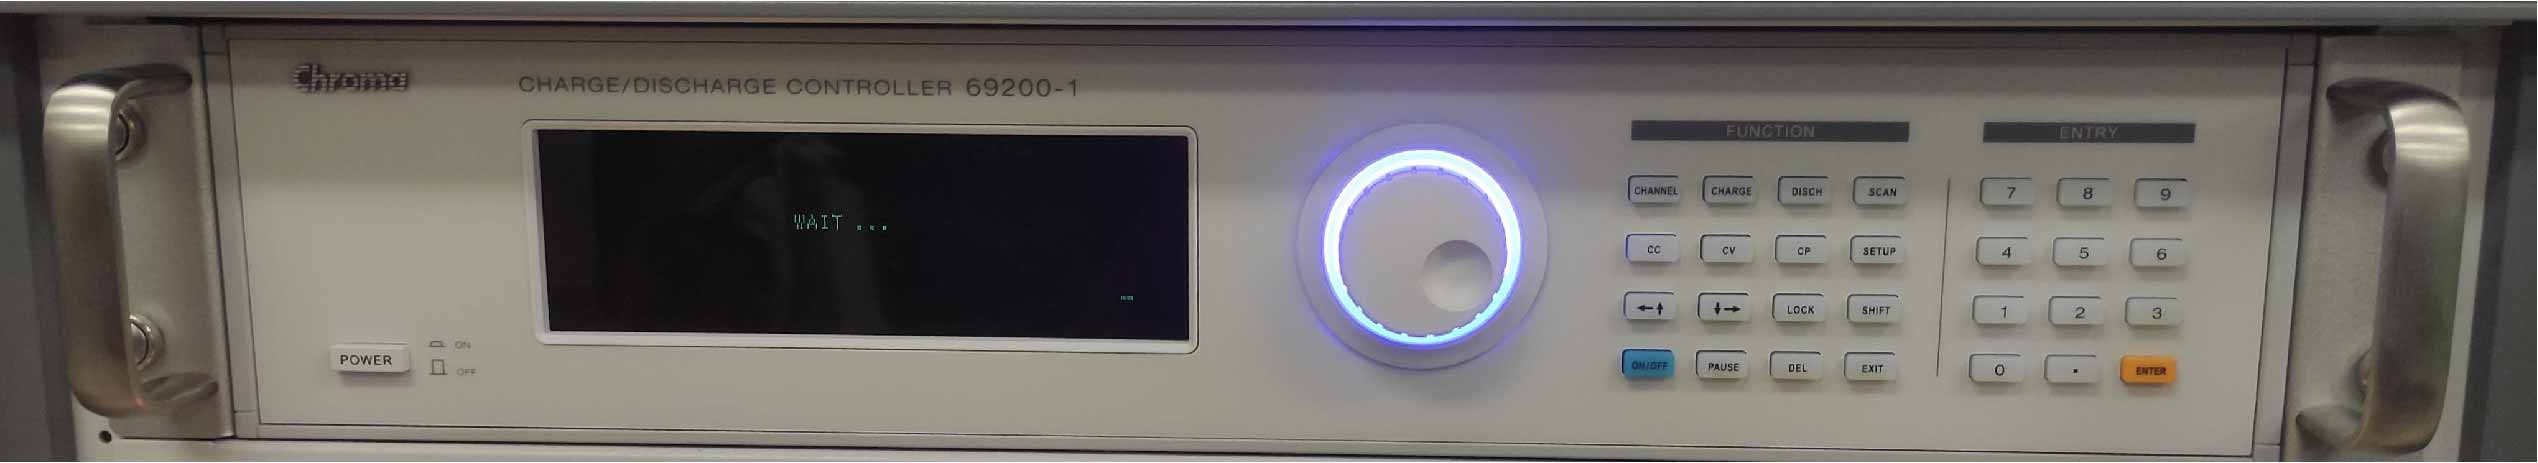
\includegraphics[width=1\linewidth]{Chapters/img/Charge_Discharge_Controller.jpg}
			\centering
			\captionsetup{justification=centering,margin=2cm}
			\caption{Charge/Discharge Controller}
	\end{figure}
	\begin{figure}[H]
		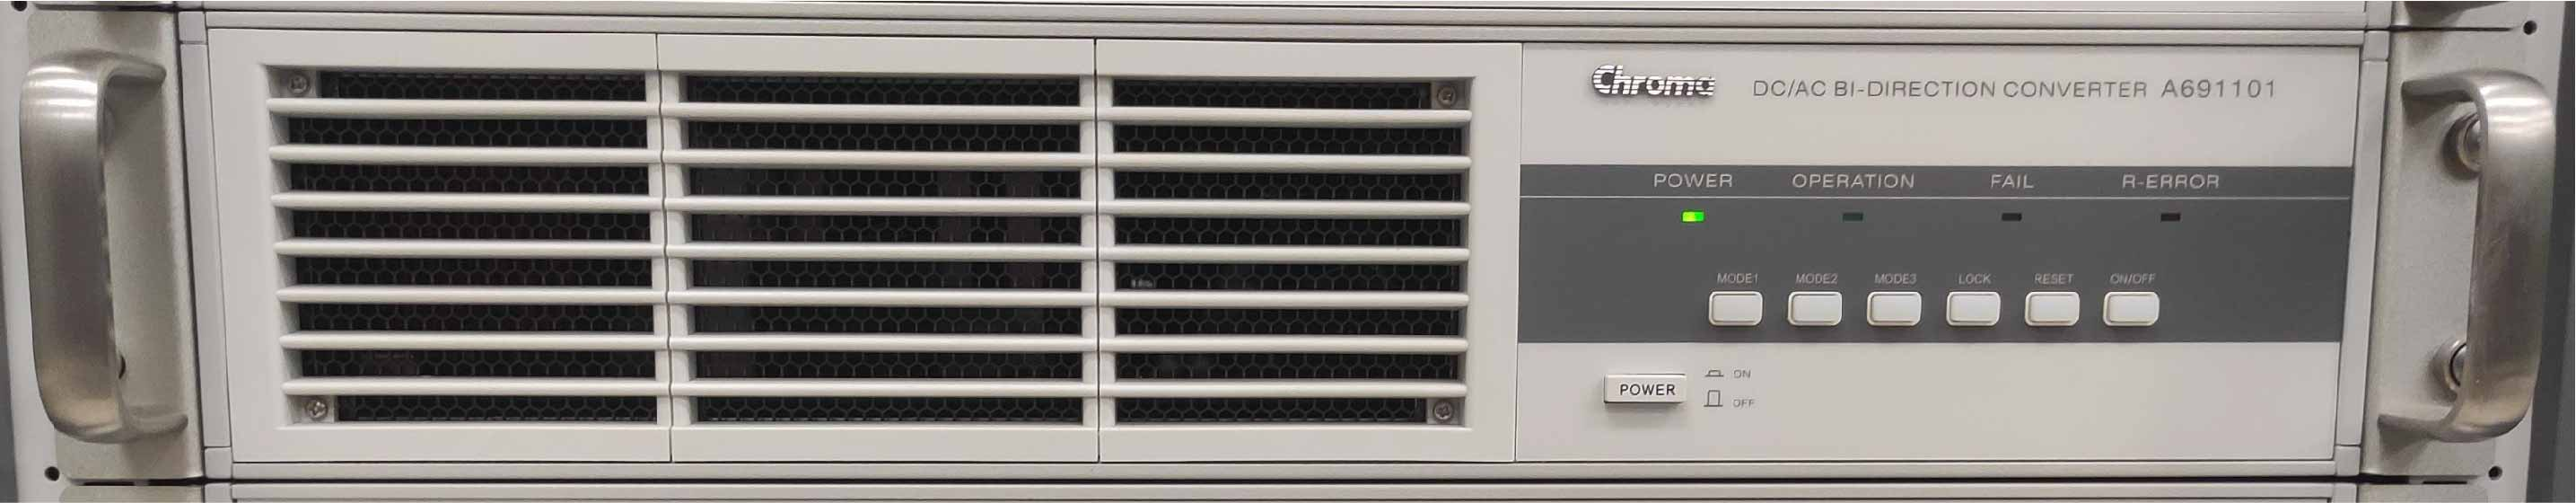
\includegraphics[width=1\linewidth]{Chapters/img/Bi_Direction_Converter.jpg}
			\centering
			\captionsetup{justification=centering,margin=2cm}
			\caption{DC/AC Bi-Direction Converter}
	\end{figure}
	\begin{figure}[H]
		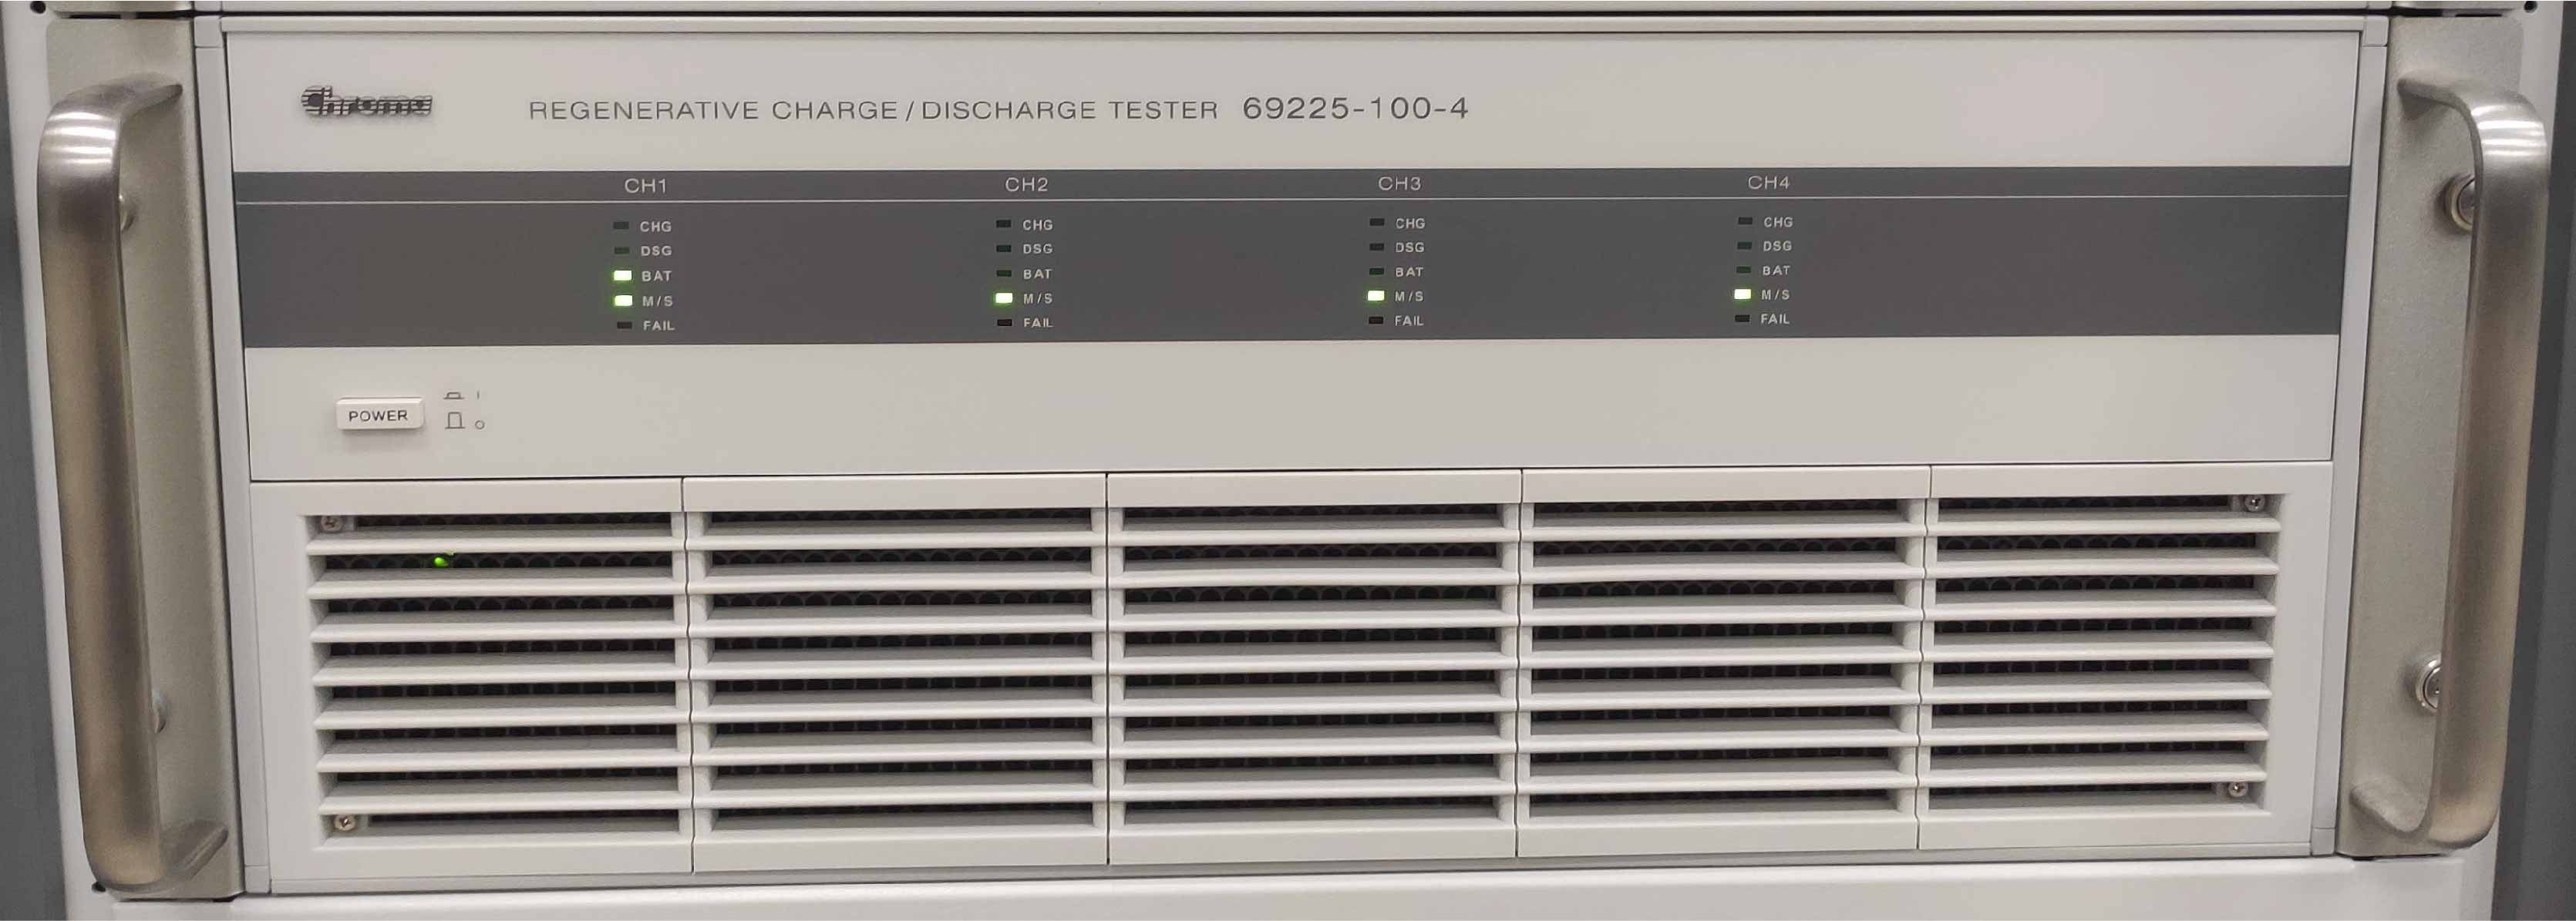
\includegraphics[width=1\linewidth]{Chapters/img/Regenerative_Charge_Discharge.jpg}
			\centering
			\captionsetup{justification=centering,margin=2cm}
			\caption{Regenerative Charge/Discharge Tester}
	\end{figure}
	\begin{figure}[H]
		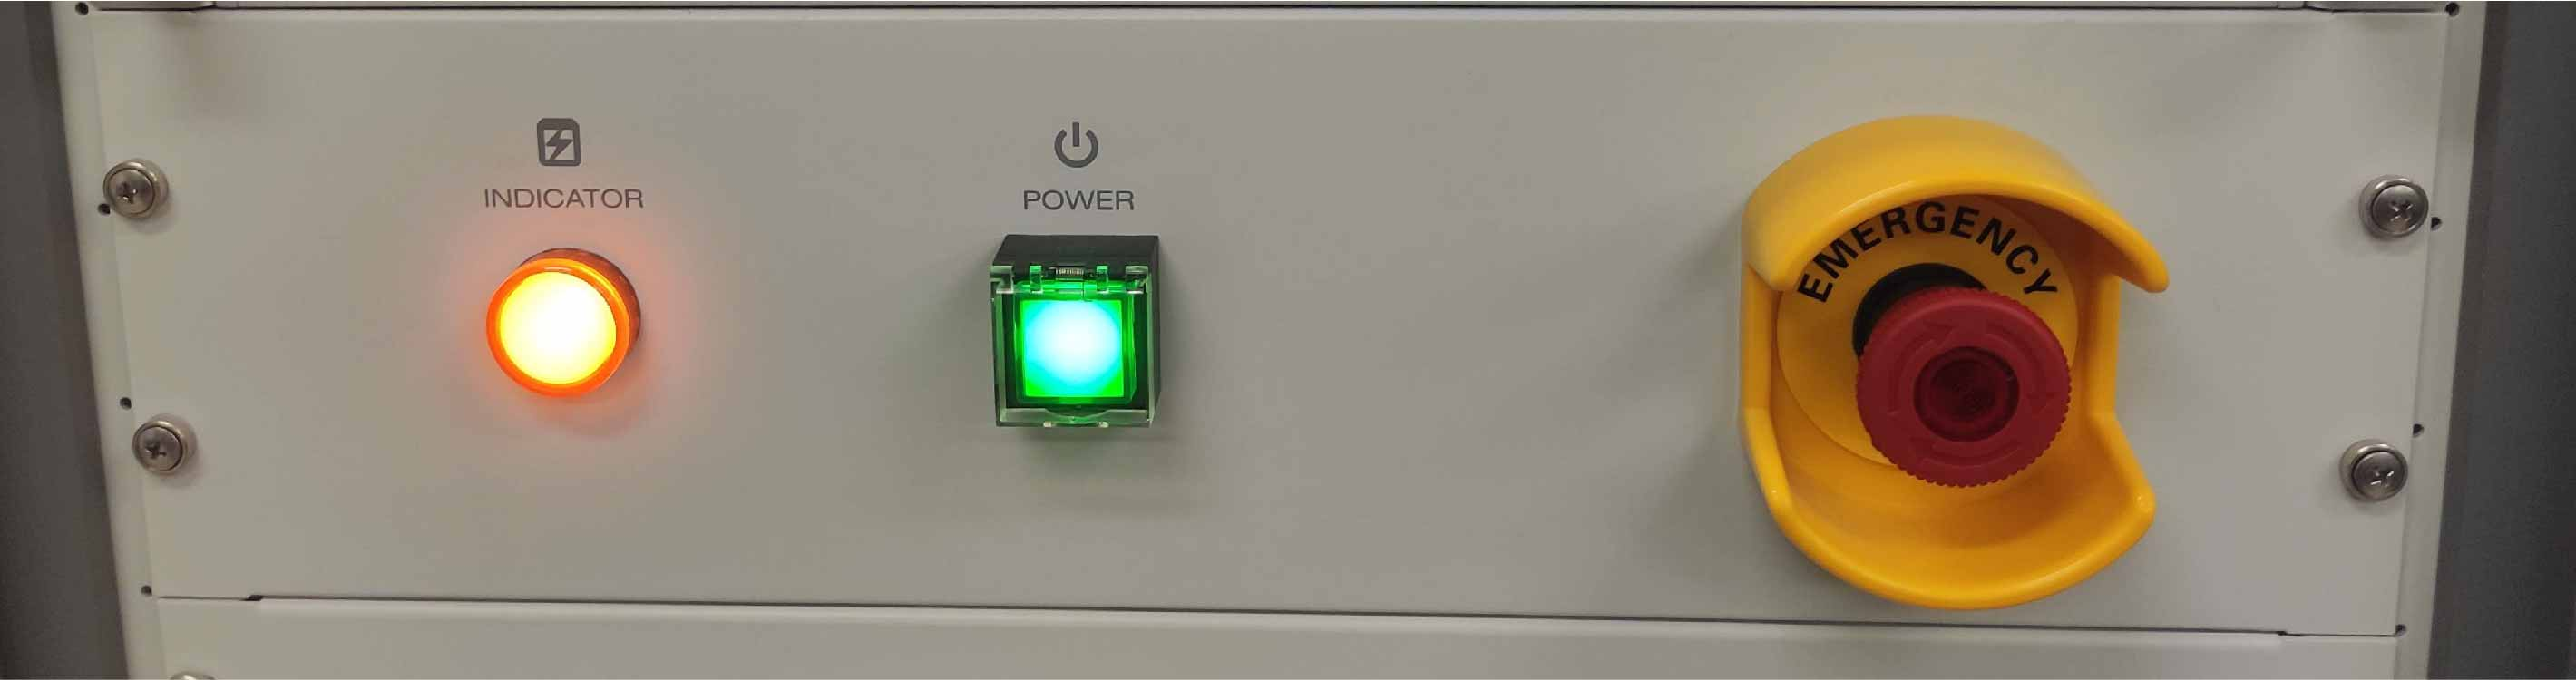
\includegraphics[width=1\linewidth]{Chapters/img/ON_OFF_Controller.jpg}
			\centering
			\captionsetup{justification=centering,margin=2cm}
			\caption{ON/OFF Controller}
	\end{figure}
%	\begin{figure}[!h]
%		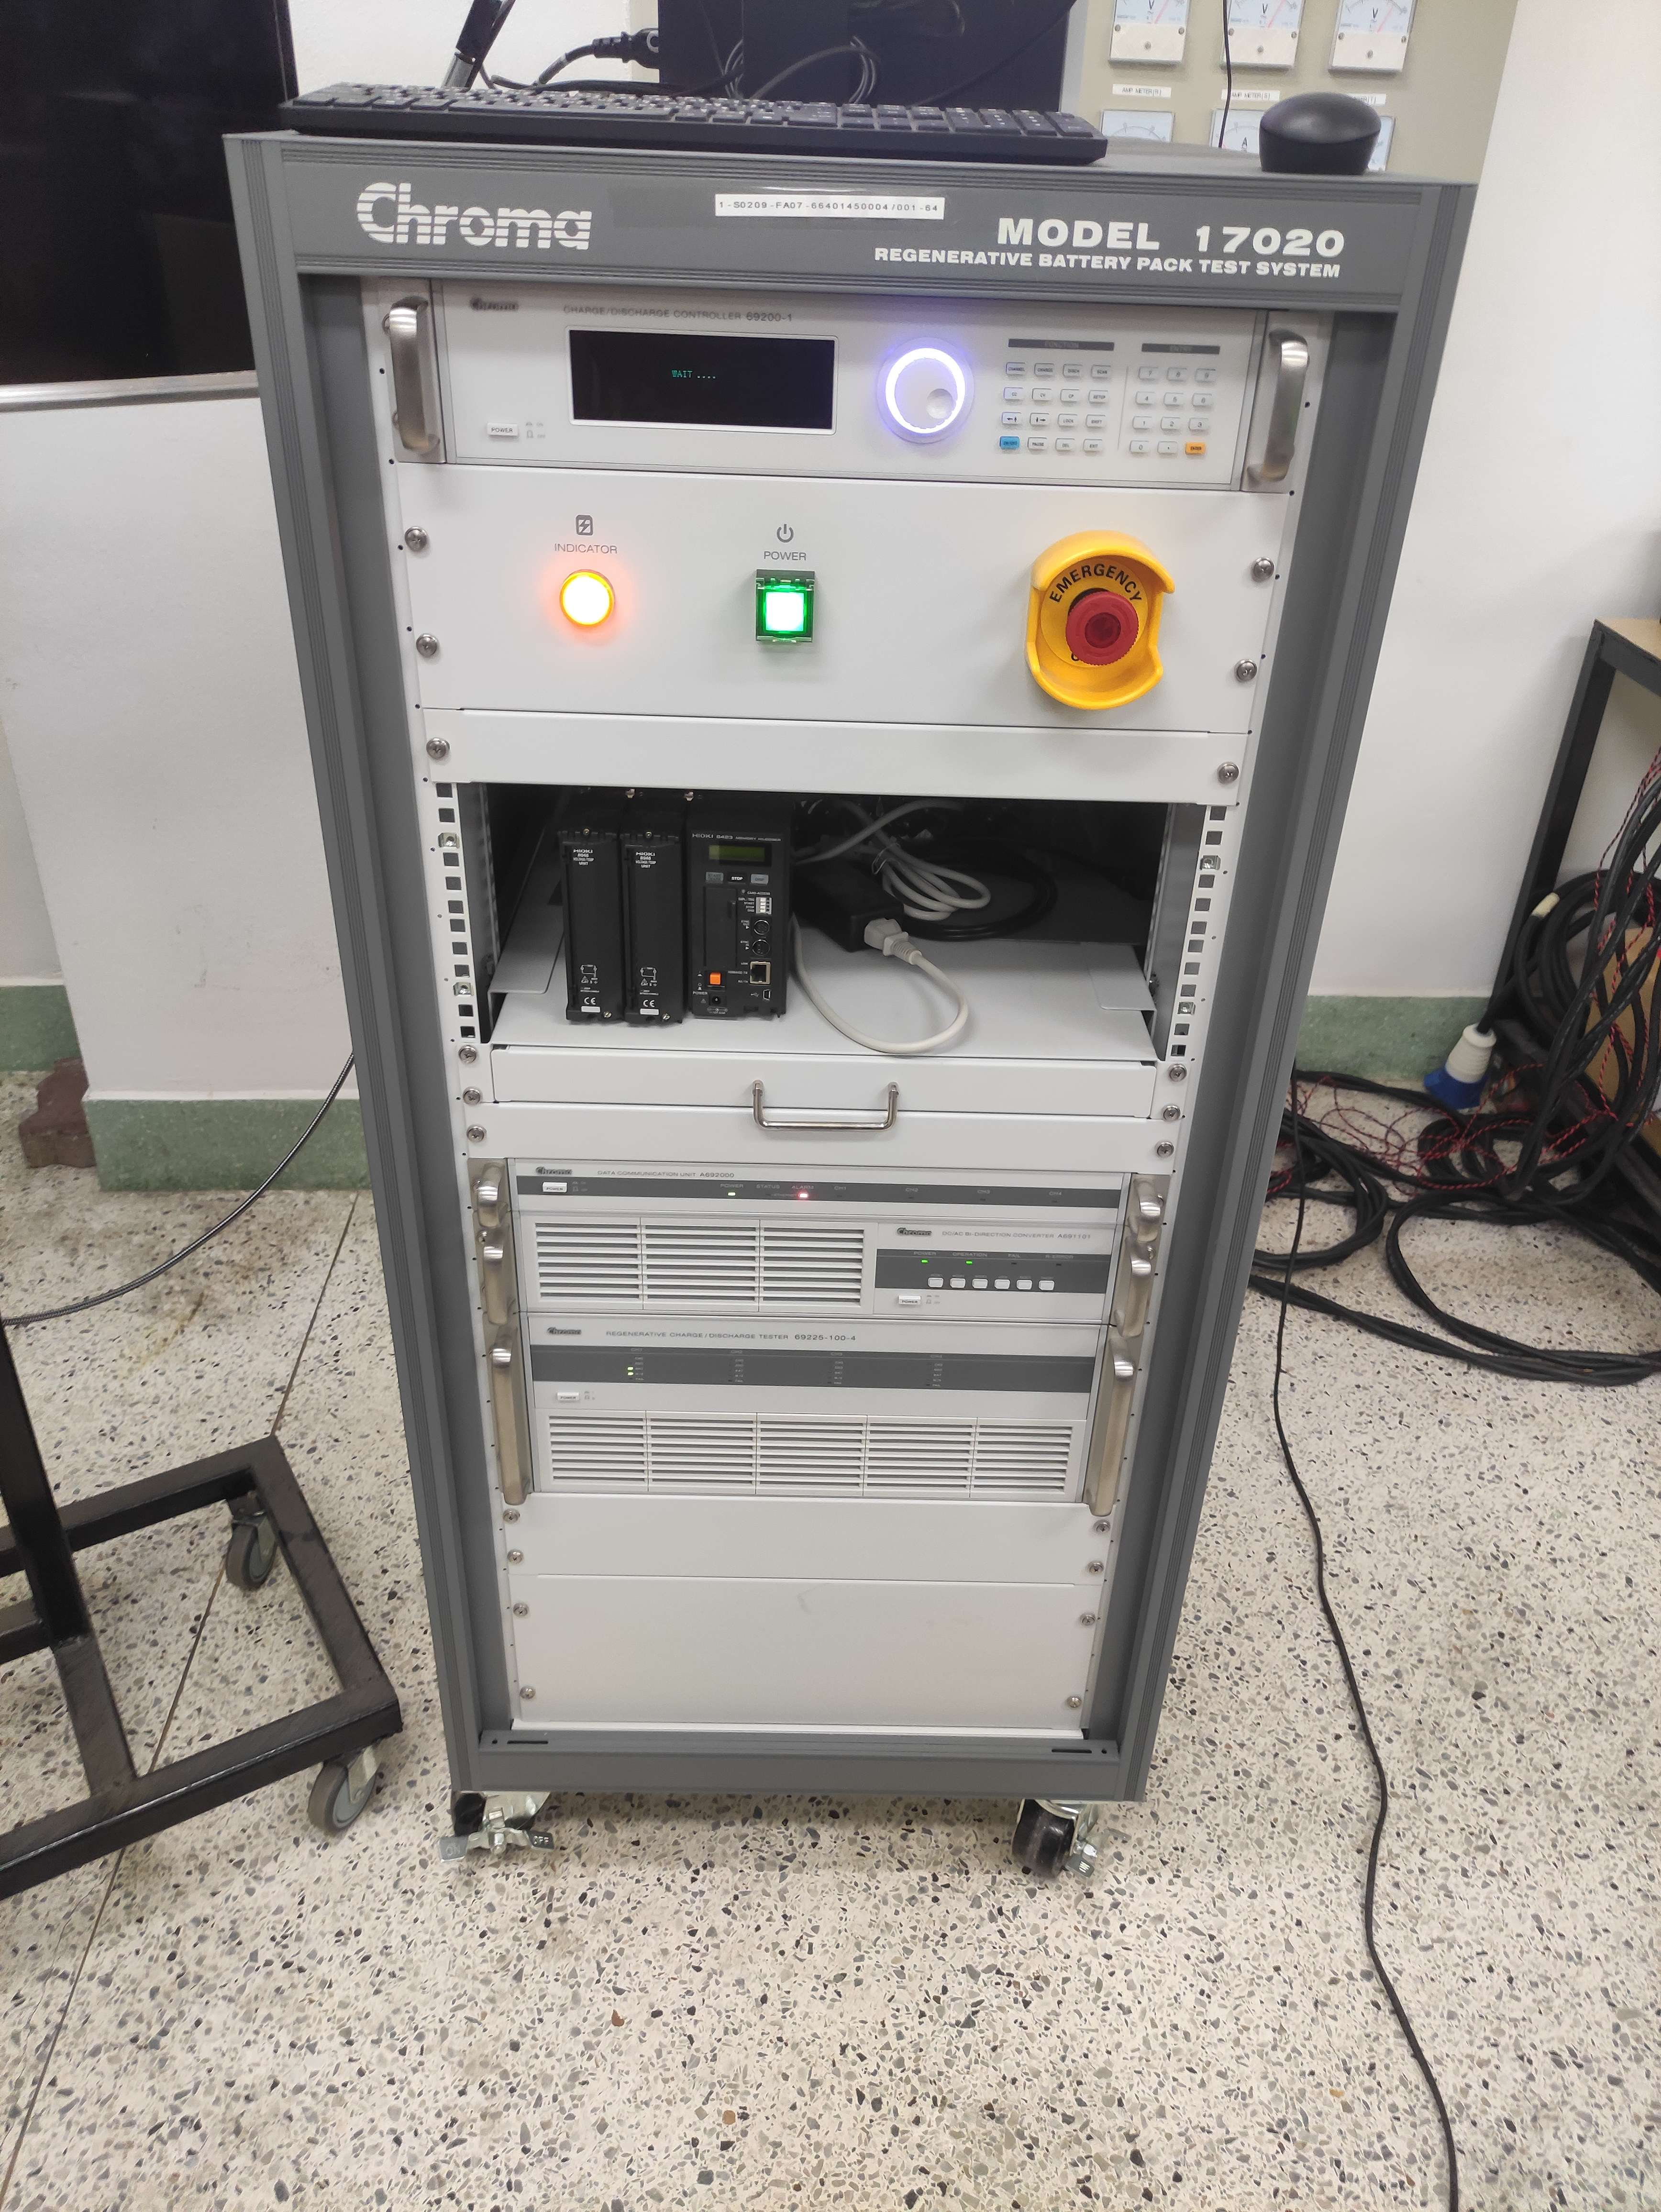
\includegraphics[width=0.5\linewidth]{Chapters/img/Chroma_17020_3.jpg}
%			\centering
%			\captionsetup{justification=centering,margin=2cm}
%			\caption{เครื่องทดสอบแบตเตอรี่ Chroma Model 17020}
%	\end{figure}
\begin{figure}[!h]
	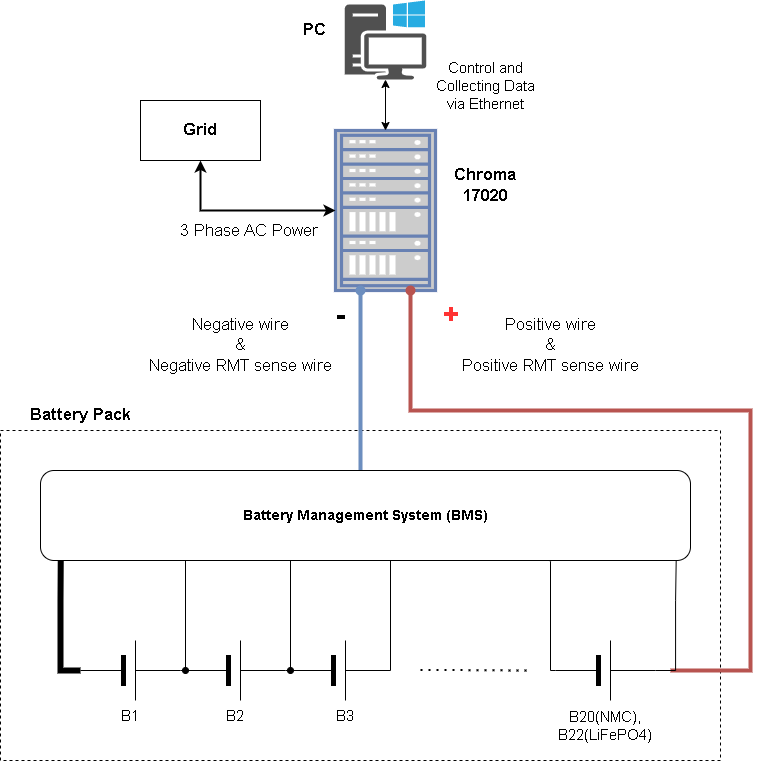
\includegraphics[width=1\linewidth]{Chapters/img/Testing_System.png}
		\centering
		\captionsetup{justification=centering,margin=2cm}
		\caption{แผนภาพระบบการทดสอบแบตเตอรี่}
		\label{fig:Testing_sys}
	\end{figure}
\end{center}
จากรูปที่\ref{fig:Testing_sys} ระบบการทดสอบนี้จะใช้คอมพิวเตอร์ในการควบคุมการทำงานของเครื่องควบคุมการชาร์จและดิสชาร์จ 69200-1 Charge/Discharge Controller โดย
เครื่องควบคุมการชาร์จและดิสชาร์จนี้จะควบคุมการชาร์จและดิสชาร์จของเครื่องทดสอบการชาร์จและดิสชาร์จ 69225-100-4 Regenerative Charge/Discharge Tester ซึ่งเครื่องทดสอบนี้
จะรับพลังงานไฟฟ้ามาจากเครื่องแปลงผันกำลังไฟฟ้า A691101 DC/AC Bi-Direction Converter เพื่อนำมาทดสอบการชาร์จและดิสชาร์จแบตเตอรี่ซึ่งผลการทดสอบจะถูกบันทึกโดยเครื่องควบคุมการชาร์จ
และดิสชาร์จและจะส่งข้อมูลผ่านระบบอีเทอร์เน็ต(Ethernet)ไปยังคอมพิวเตอร์
%========================================================================
\vfill
\subsection{แบตเตอรี่สำหรับทำการทดสอบ}
สำหรับแบตเตอรี่ที่ใช้ทำการทดสอบจะใช้แบตเตอรี่ทั้งหมด 3 โมดูลด้วยกันคือ
\begin{itemize}
 {\item แบตเตอรี่สำหรับจักรยานยนต์ไฟฟ้า 72V30Ah}
 {\item แบตเตอรี่สำหรับรถสามล้อไฟฟ้า 72V60Ah}
 {\item แบตเตอรี่ 72V72Ah}
\end{itemize}
โดยแบตเตอรี่สำหรับจักรยานยนต์ไฟฟ้าที่ใช้ทำการทดสอบเป็นโมดูลแบตเตอรี่ชนิดลิเธียมแมงกานีสโคบอลท์ออกไซด์(NMC)พิกัด 72V 30Ah ภายในโมดูลมีเซลล์แบตเตอรี่ทั้งหมด 20 เซลล์ ซึ่งแบตเตอรี่โมดูลนี้ไม่ได้มีการระบุตารางคุณสมบัติที่ชัดเจนจากผู้จำหน่ายมีเฉพาะเพียงตารางคุณสมบัติที่อยู่บนโมดูลแบตเตอรี่เท่านั้น สำหรับแบตเตอรี่สำหรับรถสามล้อไฟฟ้าพิกัด 72V 60Ah แบตเตอรี่โมดูลนี้เป็นโมดูลแบตเตอรี่ชนิดลิเธียมแมงกานีสโคบอลท์ออกไซด์(NMC)ซึ่งแบตเตอรี่โมดูลนี้ไม่ได้มีการระบุตารางคุณสมบัติที่ชัดเจนจากผู้จำหน่ายโดยทราบข้อมูลเพียงพิกัดของแบตเตอรี่เท่านั้นสุดท้าย
โมดูลแบตเตอรี่ชนิดลิเธียมฟอสเฟต(LiFePo4s)พิกัด 72V 72Ah ภายในโมดูลประกอบด้วยแบตเตอรี่จำนวน 22 เซลล์โดยตารางคุณสมบัติแสดงดังรูป\ref{table:spec_72V72Ah}

\begin{center}
%	\begin{figure}[H]
%		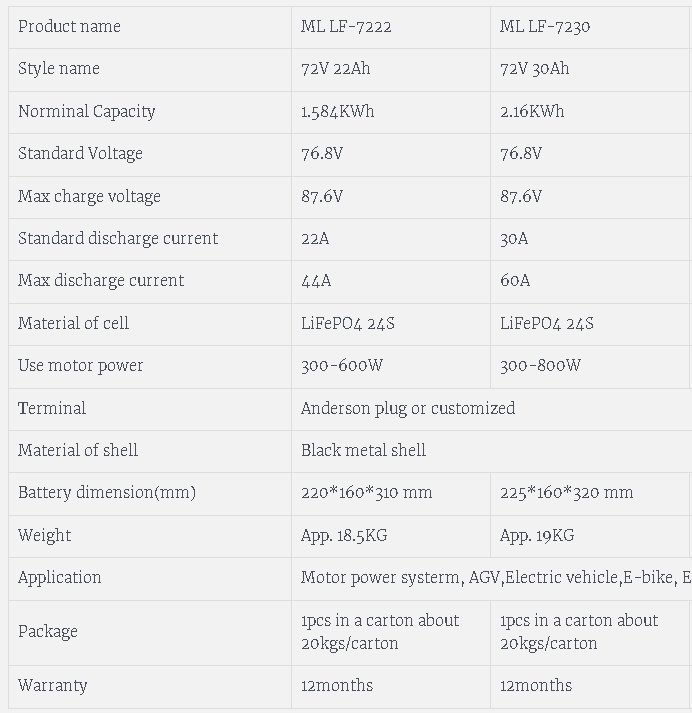
\includegraphics[width=0.5\linewidth]{Chapters/img/Battery_name_plate.PNG}
%		\centering
%		\captionsetup{justification=centering,margin=2cm}
%		\caption{ตารางคุณสมบัติของแบตเตอรี่}
%	\end{figure}
	\begin{figure}[H]
		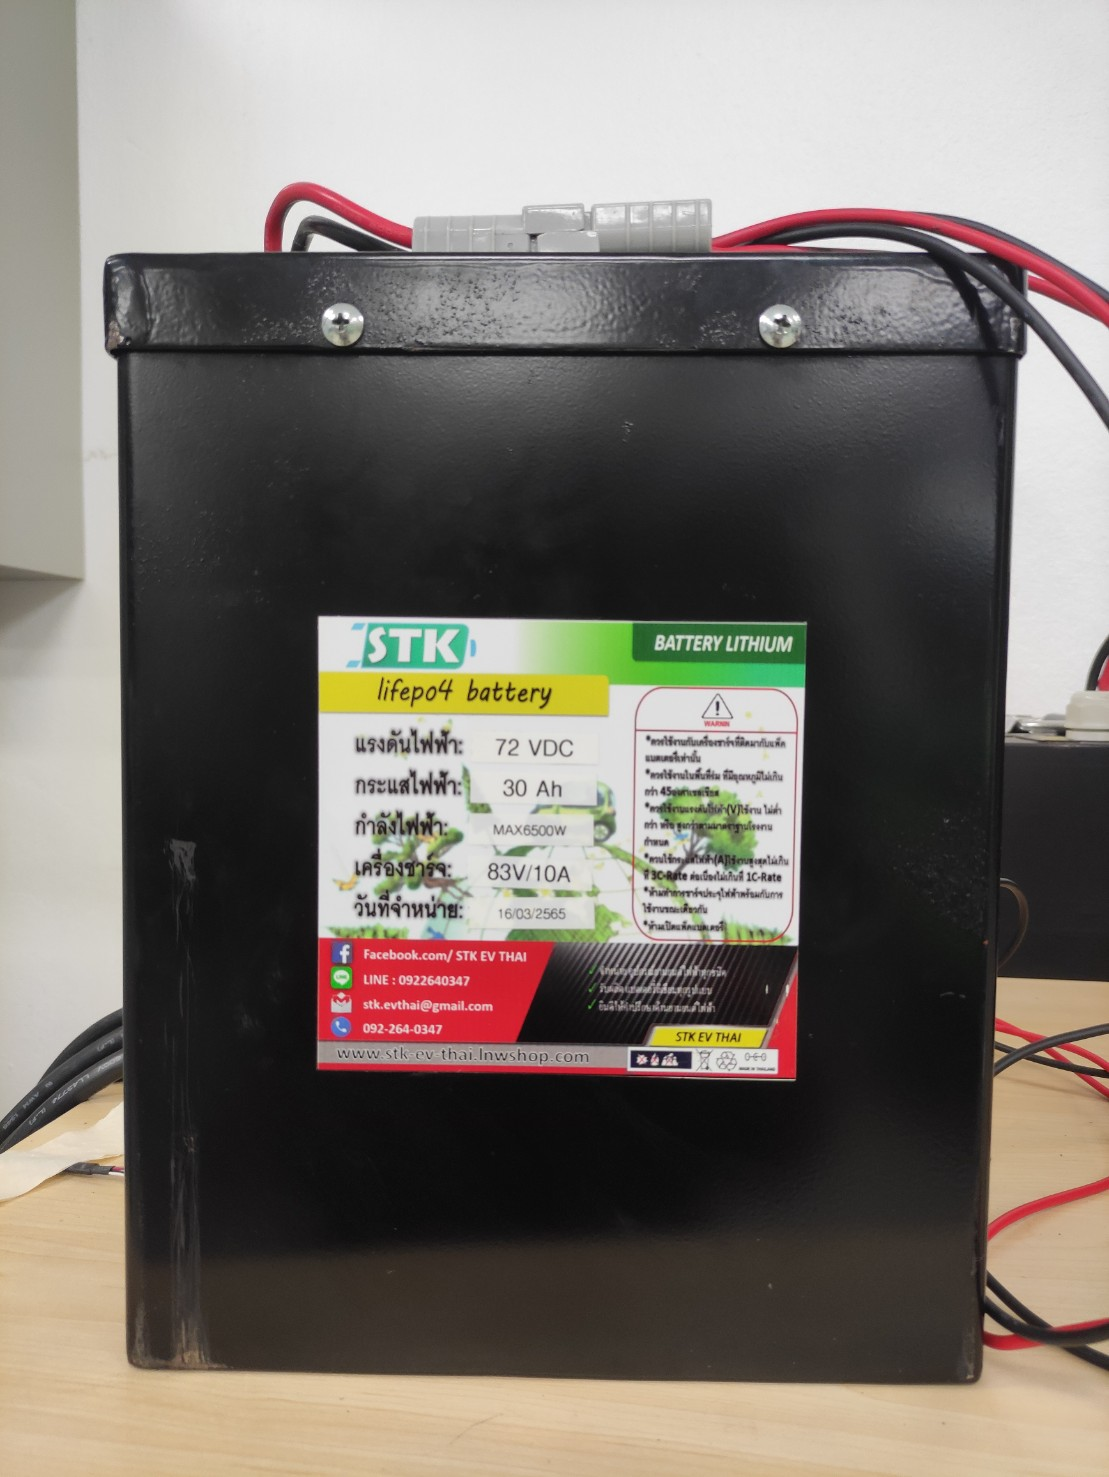
\includegraphics[width=0.5\linewidth]{Chapters/img/Battery_72V30Ah.jpg}
		\centering
		\captionsetup{justification=centering,margin=2cm}
		\caption{แบตเตอรี่สำหรับจักยานยนต์ไฟฟ้า 72V30Ah}
	\end{figure}
	\begin{figure}[H]
		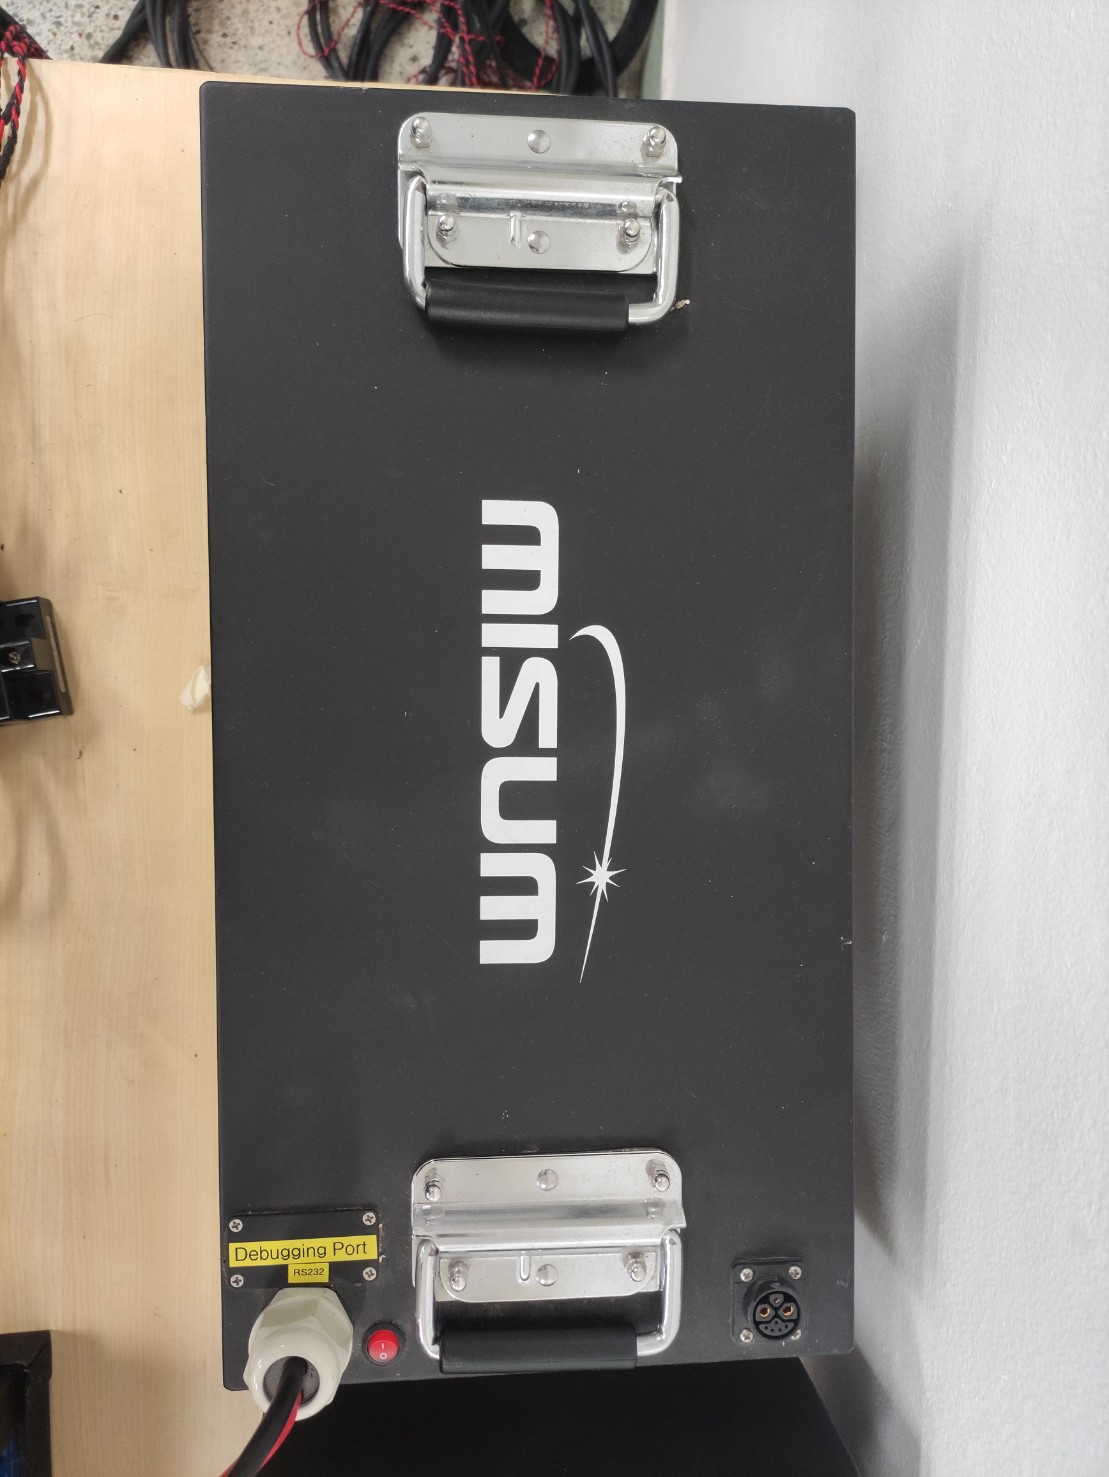
\includegraphics[width=0.5\linewidth]{Chapters/img/Battery_72V60Ah.jpg}
		\centering
		\captionsetup{justification=centering,margin=2cm}
		\caption{แบตเตอรี่สำหรับสามล้อไฟฟ้า 72V60Ah}
	\end{figure}
	\begin{figure}[H]
		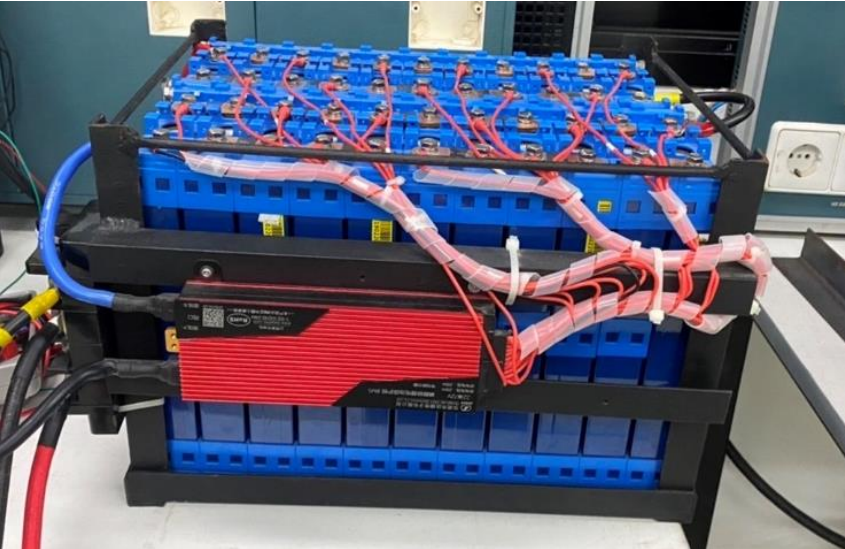
\includegraphics[width=0.5\linewidth]{Chapters/img/Battery_72V72Ah.jpg}
		\centering
		\captionsetup{justification=centering,margin=2cm}
		\caption{แบตเตอรี่ 72V72Ah}
	\end{figure}
		
\begin{table}[H]
\caption{ตารางคุณสมบัติของแบตเตอรี่ 1 เซลล์ของโมดูลแบตเตอรี่ 72V72Ah \cite{9634514}}
\centering
\resizebox{\textwidth}{!}{%
\begin{tabular}{|c|c|c|}
\hline
\textbf{Items}                & \textbf{Parameter} & \textbf{Remarks}                                              \\ \hline
Nominal Capacity              & 72Ah               & \begin{tabular}[c]{@{}c@{}}Standard \\ Discharge\end{tabular} \\ \hline
Nominal Voltage             & 3.2V      &  \\ \hline
Working Voltage             & 2.5-3.65V &  \\ \hline
Absolute Charging Voltage   & 3.8V      &  \\ \hline
Internal Resistance(Ac 1 kHz) & $\leqslant 1m\Omega$              & Fresh Cell, 30\%SOC                                           \\ \hline
Maximum charging current    & 1C        &  \\ \hline
Maximum discharging current & 2C        &  \\ \hline
Charging Time (Standard)    & $\sim$4h  &  \\ \hline
Charging Time (Fast Charge) & 1h        &  \\ \hline
SOC Window                  & 10\%-90\% &  \\ \hline
Weight                      & 1.9±0.1kg &  \\ \hline
\end{tabular}%
}
\label{table:spec_72V72Ah}
\end{table}

\end{center}
%========================================================================================================
\section{การใช้งานเครื่องทดสอบแบตเตอรี่ Chroma Model 17020}
ในหัวข้อนี้จะอธิบายถึงการใช้งานเครื่องทดสอบแบตเตอรี่ Chroma Model 17020 ขั้นตอนการใช้งานก่อนการทดสอบ เริ่มการทดสอบ และหลังจากการทดสอบโดยจะอธิบายในส่วนของเครื่องมือ(Hardware)
เป็นหลักในส่วนของโปรแกรม(Software)จะถูกอธิบายไว้ในภาคผนวก ข. โดยก่อนทำการทดสอบให้ทำการกำหนดช่องทางสำหรับการทดสอบแบตเตอรี่สำหรับเครื่องทดสอบการชาร์จและดิสชาร์จ(Regenerative Charge/Discharge Tester)จากรูปที่\ref{fig:Rear_Panel} จะเป็นส่วนด้านหลังของเครื่องทดสอบการชาร์จและดิสชาร์จโดยแต่ละส่วนของรูปมีดังนี้
\begin{enumerate}
{\item ช่องรับสัญญานจากเครื่องทดสอบการชาร์จและดิสชาร์จเครื่องอื่นผ่านสายไฟ D-Sub}
{\item ช่องส่งสัญญานจากเครื่องทดสอบการชาร์จและดิสชาร์จนี้ไปยังเครื่องทดสอบการชาร์จและดิสชาร์จอื่นผ่านสายไฟ D-Sub}
{\item สวิตซ์ชนิดมาตรฐานอินไลน์คู่(DIP Switch)สำหรับกำหนดช่องทางการทดสอบ}
{\item ช่องทางการเชื่อมต่อสาย LAN กรณีกำหนดช่องทางการทดสอบแบบขนาน}
{\item ช่องทางการเชื่อมต่อสายวัดอุณหภูมิ}
{\item ช่องทางการเชื่อมต่อสายสัญญาณชดเชยความต้านทานของสายไฟจากช่องทางการทดสอบแบตเตอรี่}
{\item ช่องทางการเชื่อมต่อสายไฟชาร์จและดิสชาร์จเพื่อทดสอบแบตเตอรี่กรณีที่กำหนดให้มีการจ่ายกระแสไฟฟ้าแบบ 2 เอาท์พุตช่องทางนี้จะใช้สำหรับเชื่อมต่อสายไฟดิสชาร์จ}
{\item ช่องทางการต่อสายไฟชาร์จเพื่อทดสอบแบตเตอรี่กรณีที่กำหนดให้มีการจ่ายกระแสไฟฟ้าแบบ 2 เอาท์พุต}
{\item ช่องทางการต่อสายไฟกระแสสลับสำหรับการให้พลังงานเครื่องทดสอบนี้}
{\item ช่องทางการต่อสายไฟกระแสตรงที่ออกจากเครื่อง A691101 DC/AC Bi-Direction Converter}
\end{enumerate}
\begin{center}
	\begin{figure}[H]
		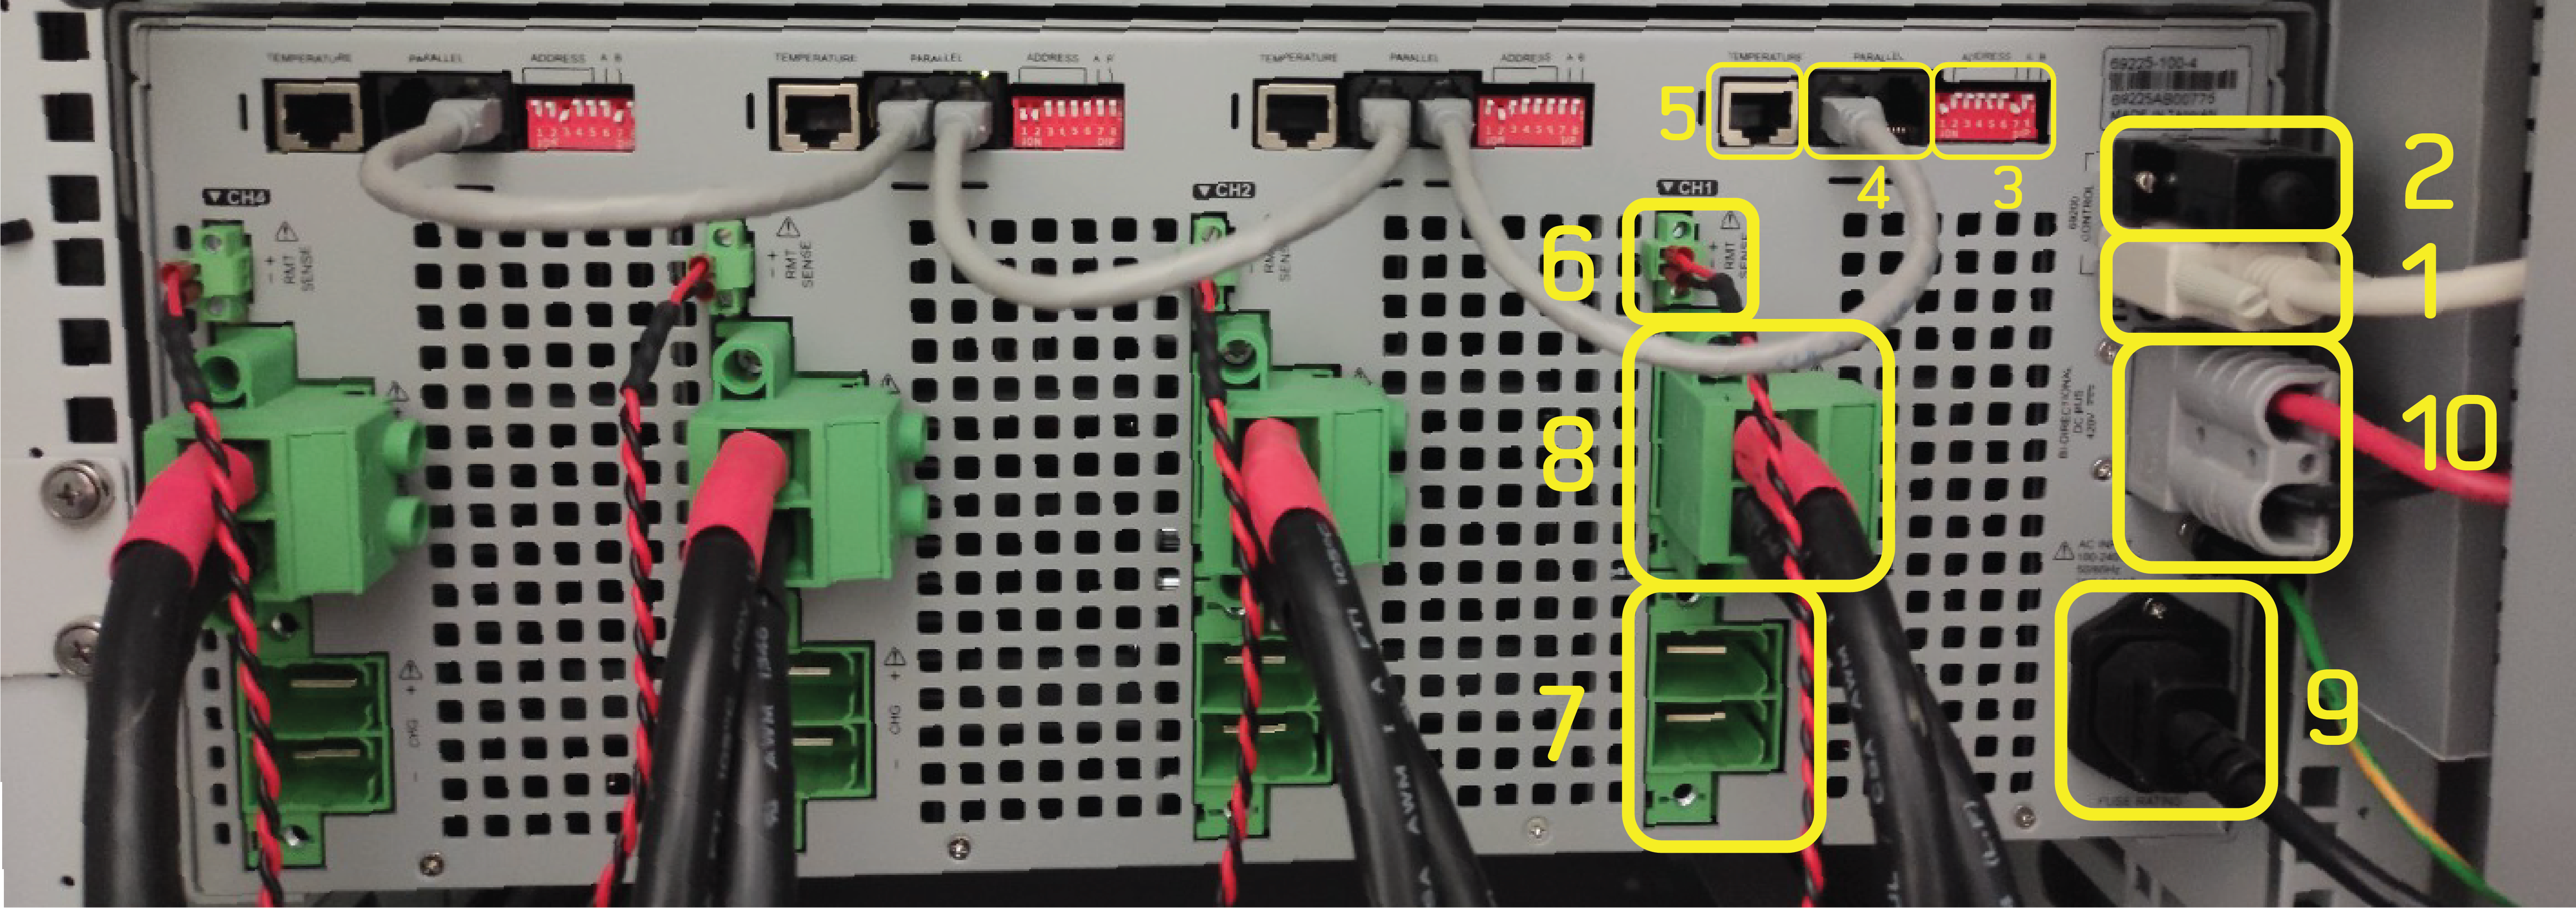
\includegraphics[width=1\linewidth]{Chapters/img/Rear_Panel_Connection.png}
		\centering
		\captionsetup{justification=centering,margin=2cm}
		\caption{ด้านหลังของเครื่องทดสอบการชาร์จและดิสชาร์จ}
		\label{fig:Rear_Panel}
	\end{figure}
	\begin{figure}[H]
		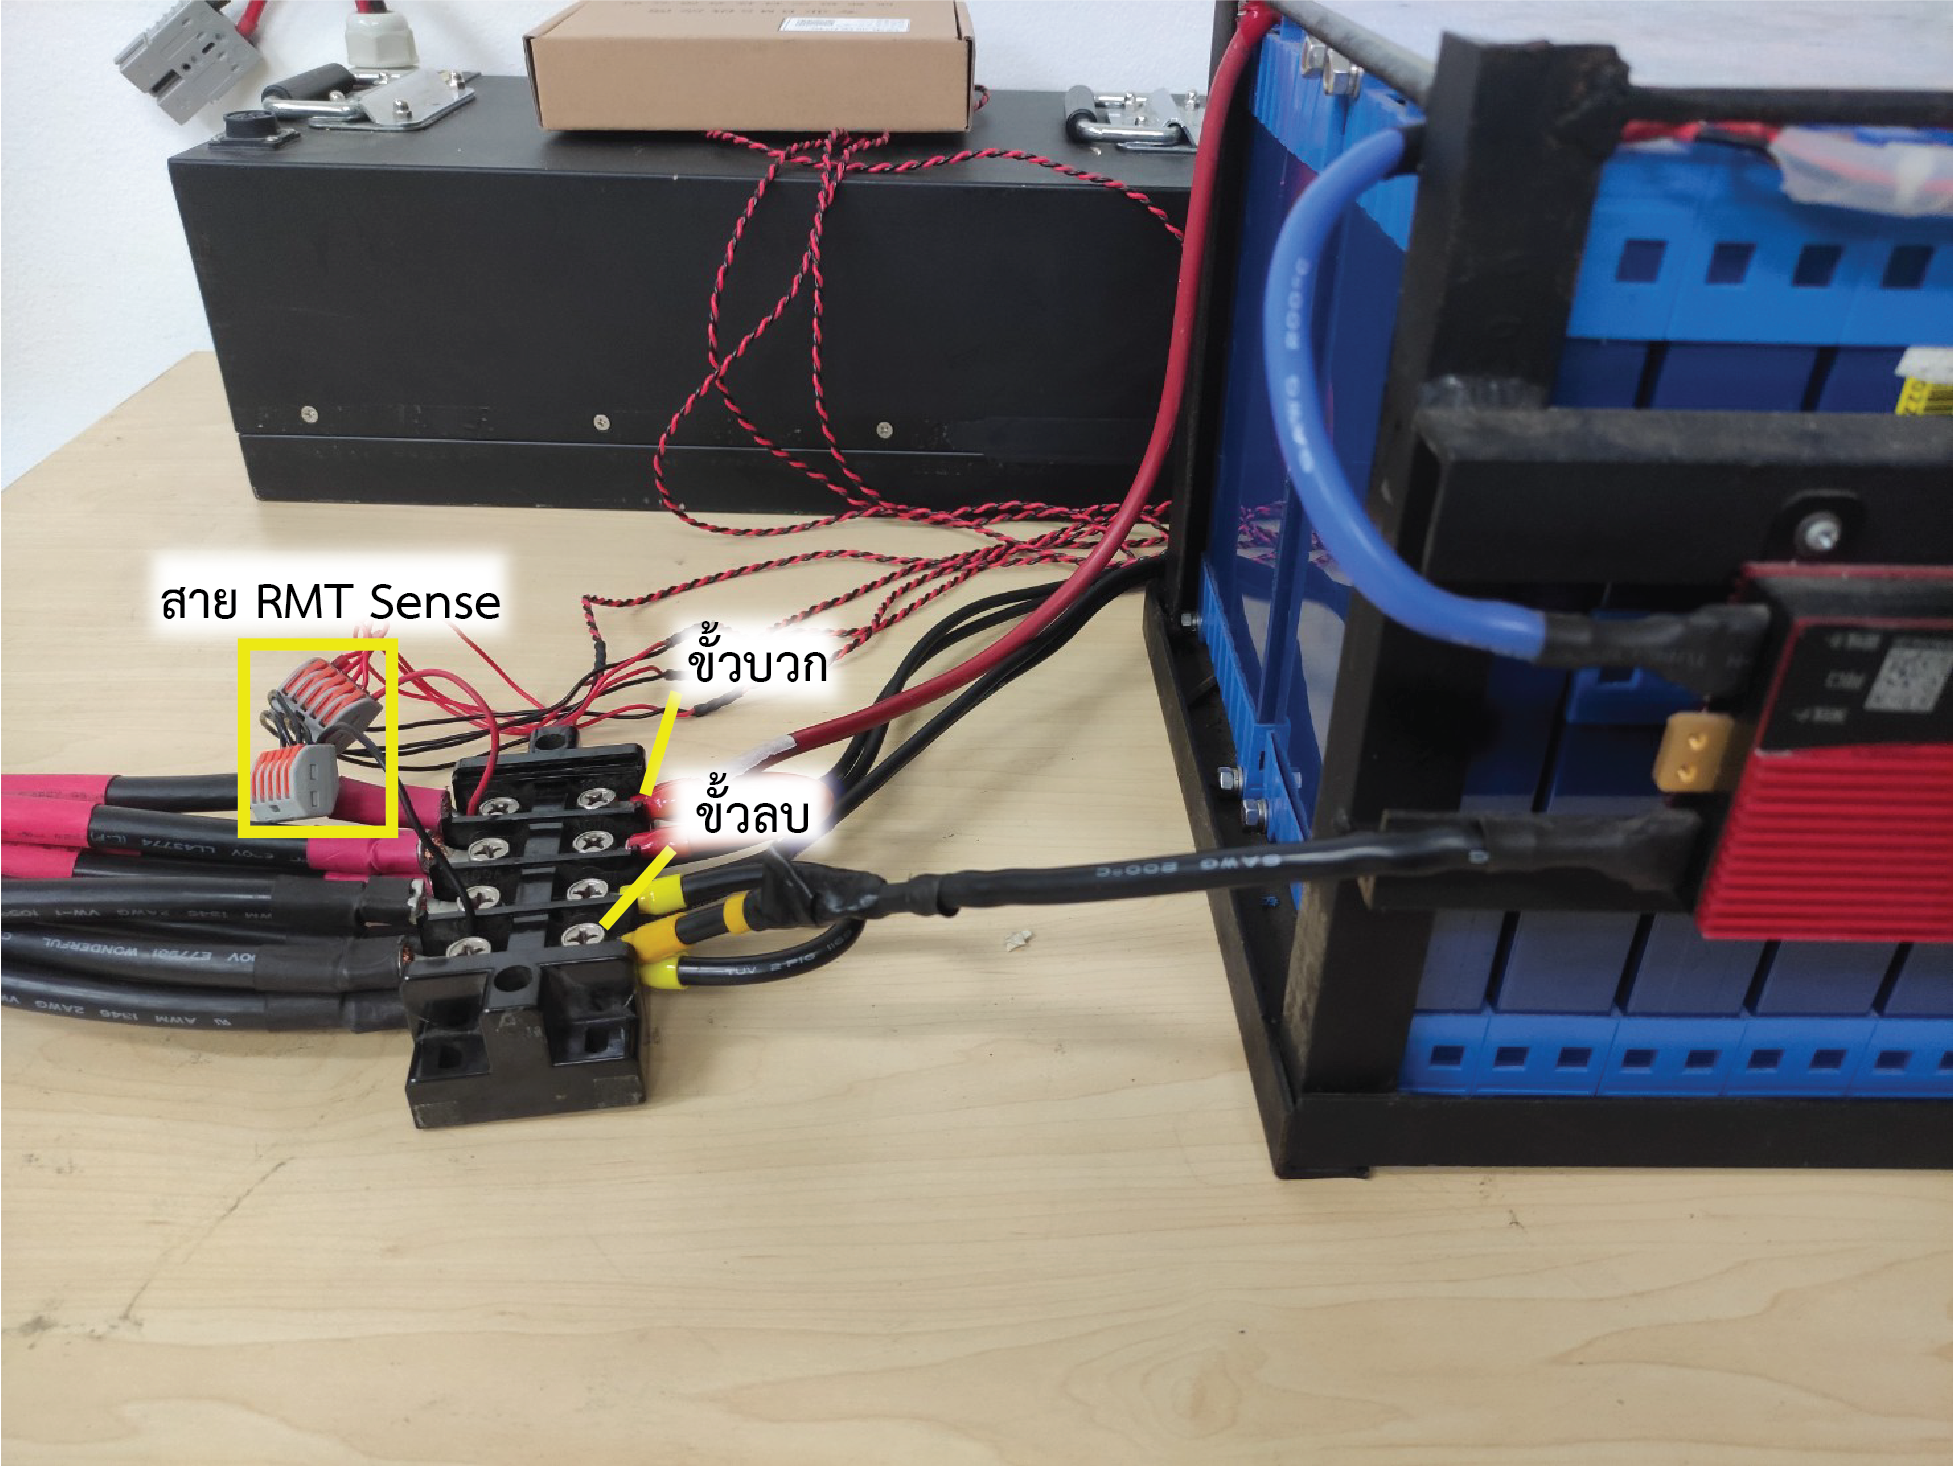
\includegraphics[width=1\linewidth]{Chapters/img/Wire_Conn.png}
		\centering
		\captionsetup{justification=centering,margin=2cm}
		\caption{การเชื่อมต่อแบตเตอรี่กับเครื่องทดสอบแบตเตอรี่ Chroma 17020}
		\label{fig:Wire_Conn}
	\end{figure}
\end{center}
\begin{table}[H]
\caption{แนวทางการกำหนดช่องทางการทดสอบ}
\centering
\begin{tabular}{ |p{5cm}||p{1cm}||p{2.5cm}||p{3cm}|  }
 \hline
 \multicolumn{4}{|c|}{ตารางการกำหนดช่องทางการทดสอบ} \\
 \hline
 เลือกช่องทาง &NC(8) & Parallel(7) & Adress(6,5,4,3,2,1)\\
 \hline
 ช่องทางที่1แบบไม่ขนาน &0 & 0& 00001\\
 ช่องทางที่2แบบไม่ขนาน &0 & 0& 00010\\
 ช่องทางที่3แบบไม่ขนาน &0 & 0& 00011\\
 ช่องทางที่4แบบไม่ขนาน &0 & 0& 00100\\
 \hline
 ช่องทางที่1แบบขนาน &0 & 1& 00001\\
 ช่องทางที่2แบบขนาน &0 & 1& 00010\\
 ช่องทางที่3แบบขนาน &0 & 1& 00011\\
 ช่องทางที่4แบบขนาน &0 & 1& 00100\\
 \hline
 \end{tabular}
\label{tab:select_table}
\end{table}

สำหรับส่วนที่ 3 ซึ่งจะเป็นส่วนที่ต้องทำการกำหนดช่องทางการทดสอบโดยขึ้นอยู่กับการเปิด ปิดของสวิตซ์ชนิดมาตรฐานอินไลน์คู่(DIP Switch)
โดยแนวทางการกำหนดช่องทางการทดสอบจะเป็นไปดังตารางที่\ref{tab:select_table} ซึ่งจะสังเกตได้ว่าการกำหนดช่องทางการทดสอบนั้นจะใช้การระบุ
เป็นเลข-ฐาน 2 สำหรับกรณีที่เป็นการกำหนดช่องทางแบบขนานจะต้องทำการเชื่อมต่อสาย LAN ระหว่างช่องทางดังรูปที่\ref{fig:Rear_Panel} เมื่อกำหนดช่องทางการทดสอบได้แล้วให้ทำการเชื่อมต่อแบตเตอรี่สำหรับการทดสอบกับช่องทางการทดสอบที่ได้กำหนดไว้ดังรูป\ref{fig:Wire_Conn} และเชื่อมต่อสายสัญญาณชดเชยความต้านทานของสายไฟจากช่องทางการทดสอบแบตเตอรี่เข้ากับแบตเตอรี่โดยสายสีแดงให้เชื่อมต่อกับขั้วบวกของแบตเตอรี่ส่วนสายสีดำให้เชื่อมต่อกับขั้วลบ
ของแบตเตอรี่ซึ่งในกรณีที่มีการกำหนดช่องทางการทดสอบแบตเตอรี่เป็นแบบขนานให้เชื่อมต่อสายชดเชยนี้แบบขนานด้วยเช่นกันดังรูปที่\ref{fig:Wire_Conn}
จากนั้นให้ทำการดำเนินเครื่องทดสอบโดยตรวจสอบในส่วนของเครื่องควบคุมการจ่ายไฟฟ้า(ON/OFF Controller)
ถ้าหากเครื่องทดสอบได้รับกระแสไฟฟ้าจะเห็นได้ว่าจะแสดงไฟสถานะสีเหลืองดังรูปที่\ref{fig:Indicator_light}ถ้าหากเครื่องควบคุมมีการแสดงไฟสถานะสีแดงดังรูป\ref{fig:Emergency_stop} นั่นหมายความว่าเครื่องควบคุมยังอยู่ในสถานะหยุดการทำงานฉุกเฉินให้ทำการหมุนสวิตซ์สีแดงไปทางขวาเพื่อให้เครื่องควบคุมออกจากสถานะดังกล่าวจากนั้นเครื่องควบคุมจะแสดงเพียงสถานะไฟสีเหลืองดังเดิม จากนั้นให้ทำการกดสวิตซ์สีเขียวเพื่อให้เครื่องควบคุมทำการจ่ายกระแสไฟฟ้าในกับส่วนอื่นๆของระบบเมื่อกดสวิตซ์แล้วเครื่องควบคุมจะแสดงไฟสถานะสีเขียวดังรูปที่\ref{fig:Power_button}
จากนั้นให้ทำการสังเกตไฟสถาณะที่ส่วนอื่นๆของระบบถ้าหากไม่มีการแสดงไฟสถานะให้ทำการดำเนินเครื่องมืออื่นๆในระบบต่อไปโดยการกดสวิตซ์ดำเนินเครื่อง
\newline 
\hspace*{2cm}
ข้างต้นเป็นขั้นตอนก่อนการเริ่มการทดสอบซึ่งในส่วนของโปรแกรมจะใช้การตั้งค่า UUT Setup 
ดังรูปที่\ref{UUT2} - \ref{UUT3}ทุกส่วนของโปรแกรมการทดสอบในโครงงานนี้ซึ่งสำหรับการตั้งค่าอื่นๆจะกล่าวในหัวข้อถัดๆไป
\begin{center}
	\begin{figure}[H]
		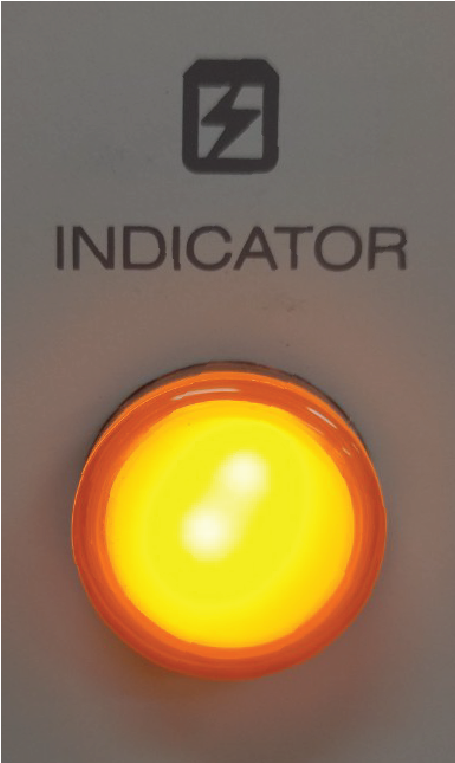
\includegraphics[width=0.25\linewidth]{Chapters/img/Indicator.png}
		\centering
		\captionsetup{justification=centering,margin=2cm}
		\caption{ไฟแสดงสถานะขณะมีกระแสไฟฟ้าภายในเครื่องทดสอบ}
		\label{fig:Indicator_light}
	\end{figure}
	\begin{figure}[H]
		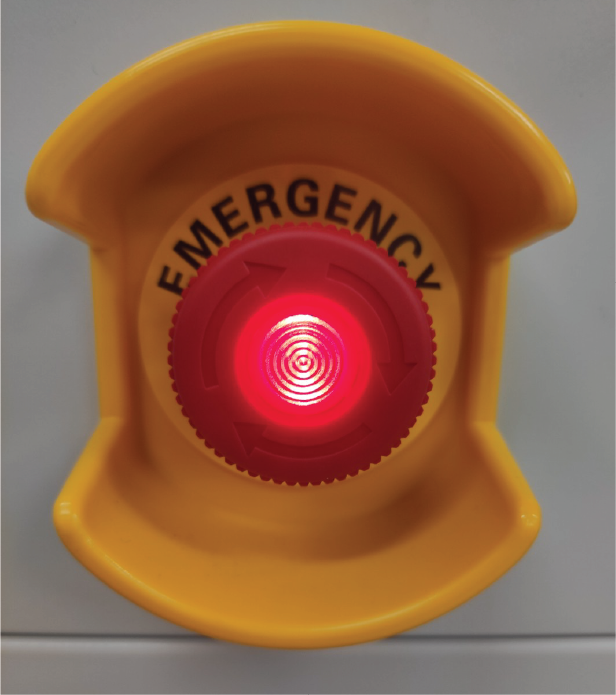
\includegraphics[width=0.25\linewidth]{Chapters/img/Emergency_stop.png}
		\centering
		\captionsetup{justification=centering,margin=2cm}
		\caption{สวิตซ์หยุดฉุกเฉินและไฟแสดงสถานะหยุดฉุกเฉิน}
		\label{fig:Emergency_stop}
	\end{figure}
	\begin{figure}[H]
		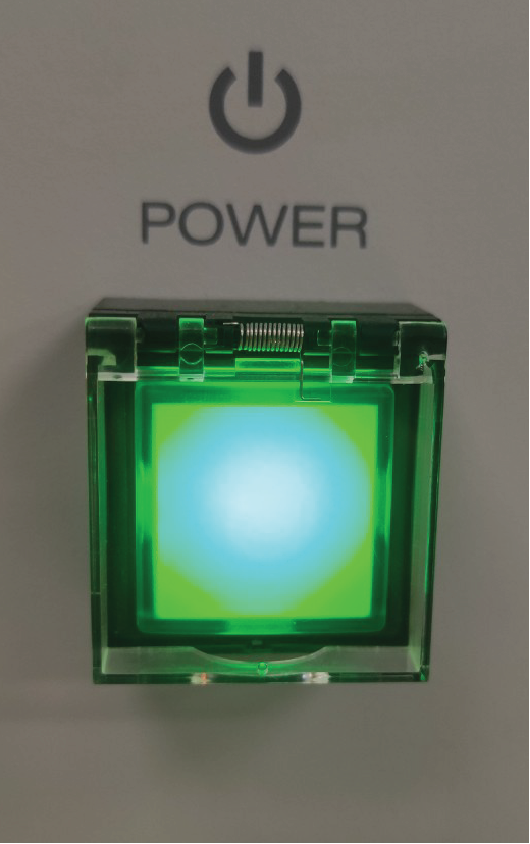
\includegraphics[width=0.25\linewidth]{Chapters/img/Power_Button.png}
		\centering
		\captionsetup{justification=centering,margin=2cm}
		\caption{สวิตซ์ดำเนินเครื่องทดสอบและไฟสถานะแสดงความพร้อมการใช้งาน}
		\label{fig:Power_button}
	\end{figure}
	\begin{figure}[H]
	\makebox[\textwidth]{
	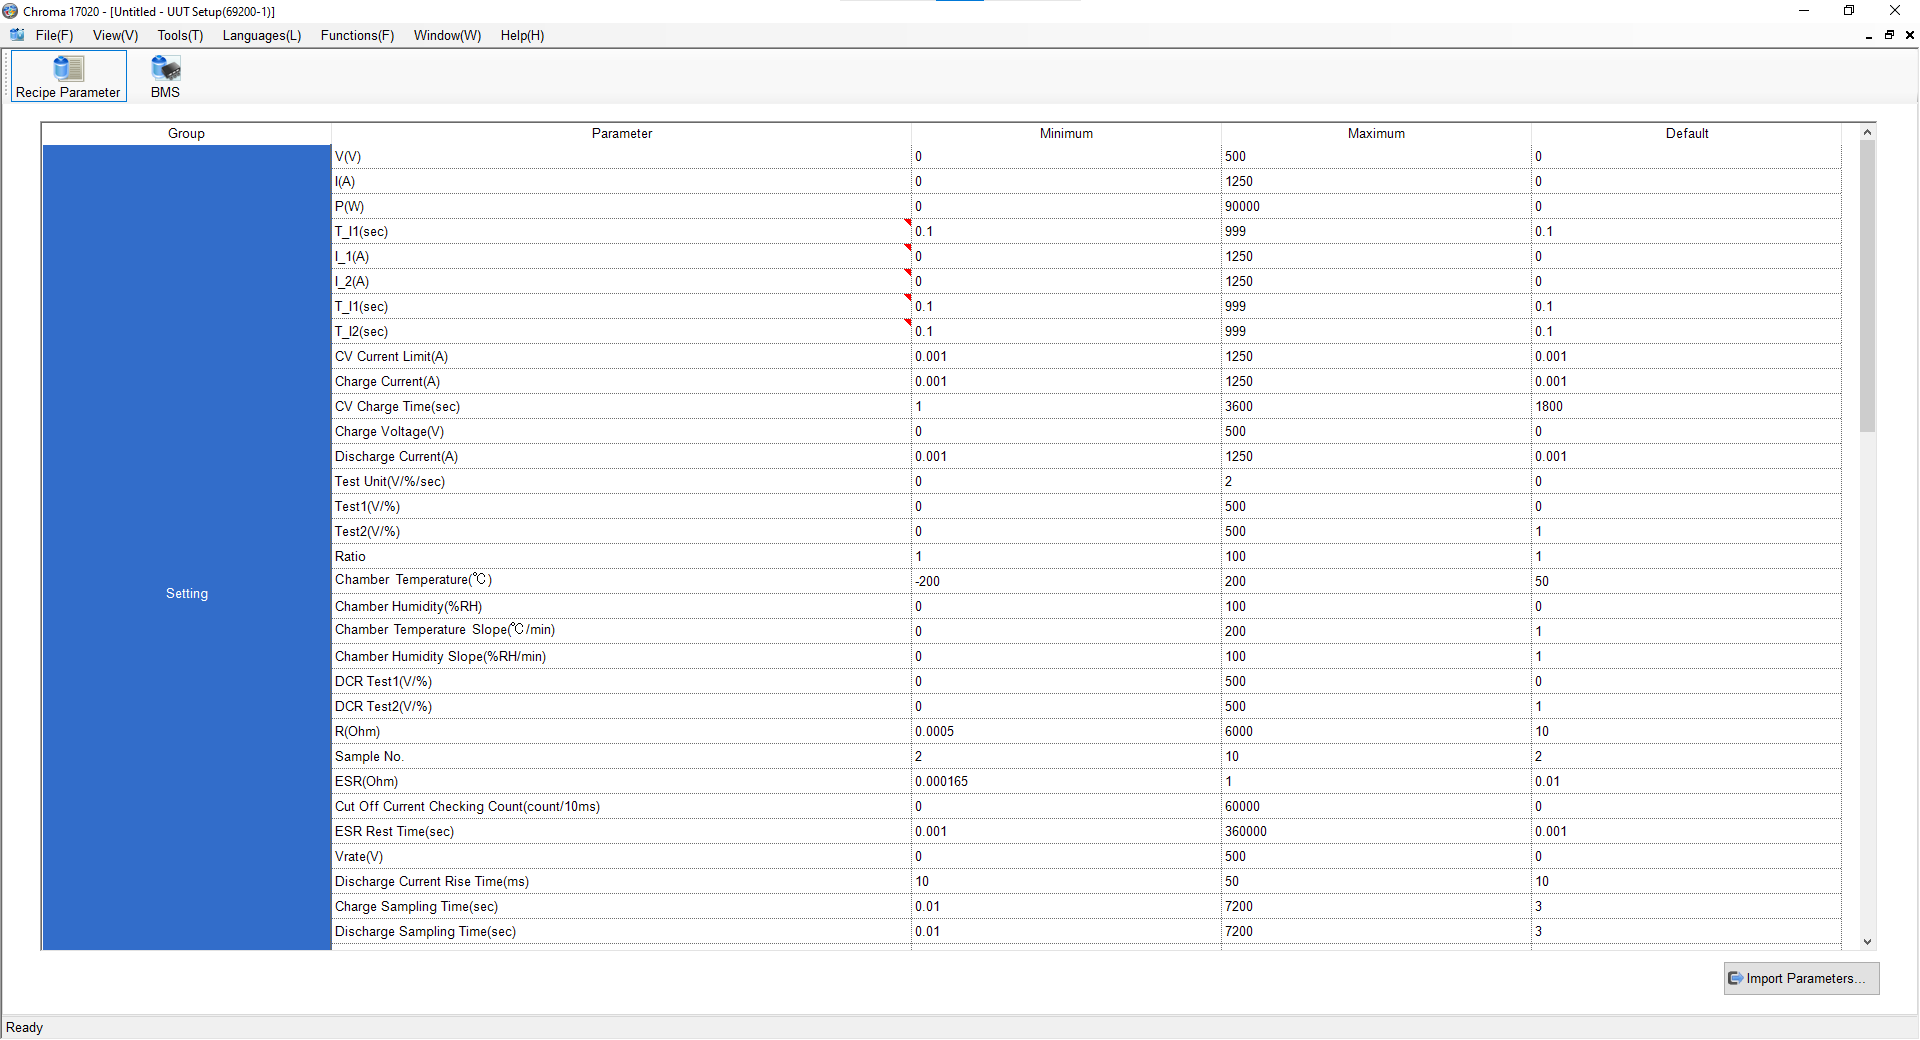
\includegraphics[width=0.8\paperwidth]{Chapters/img/R136_DEMO/UUT_SETUP_1.png}}
		\centering
		\captionsetup{justification=centering,margin=2cm}
		\caption{การกำหนดขอบเขตตัวแปรต่างๆใน UUT Setup (ก)}
		\label{fig:UUT1}
	\end{figure}
	\begin{figure}[H]
	\makebox[\textwidth]{
	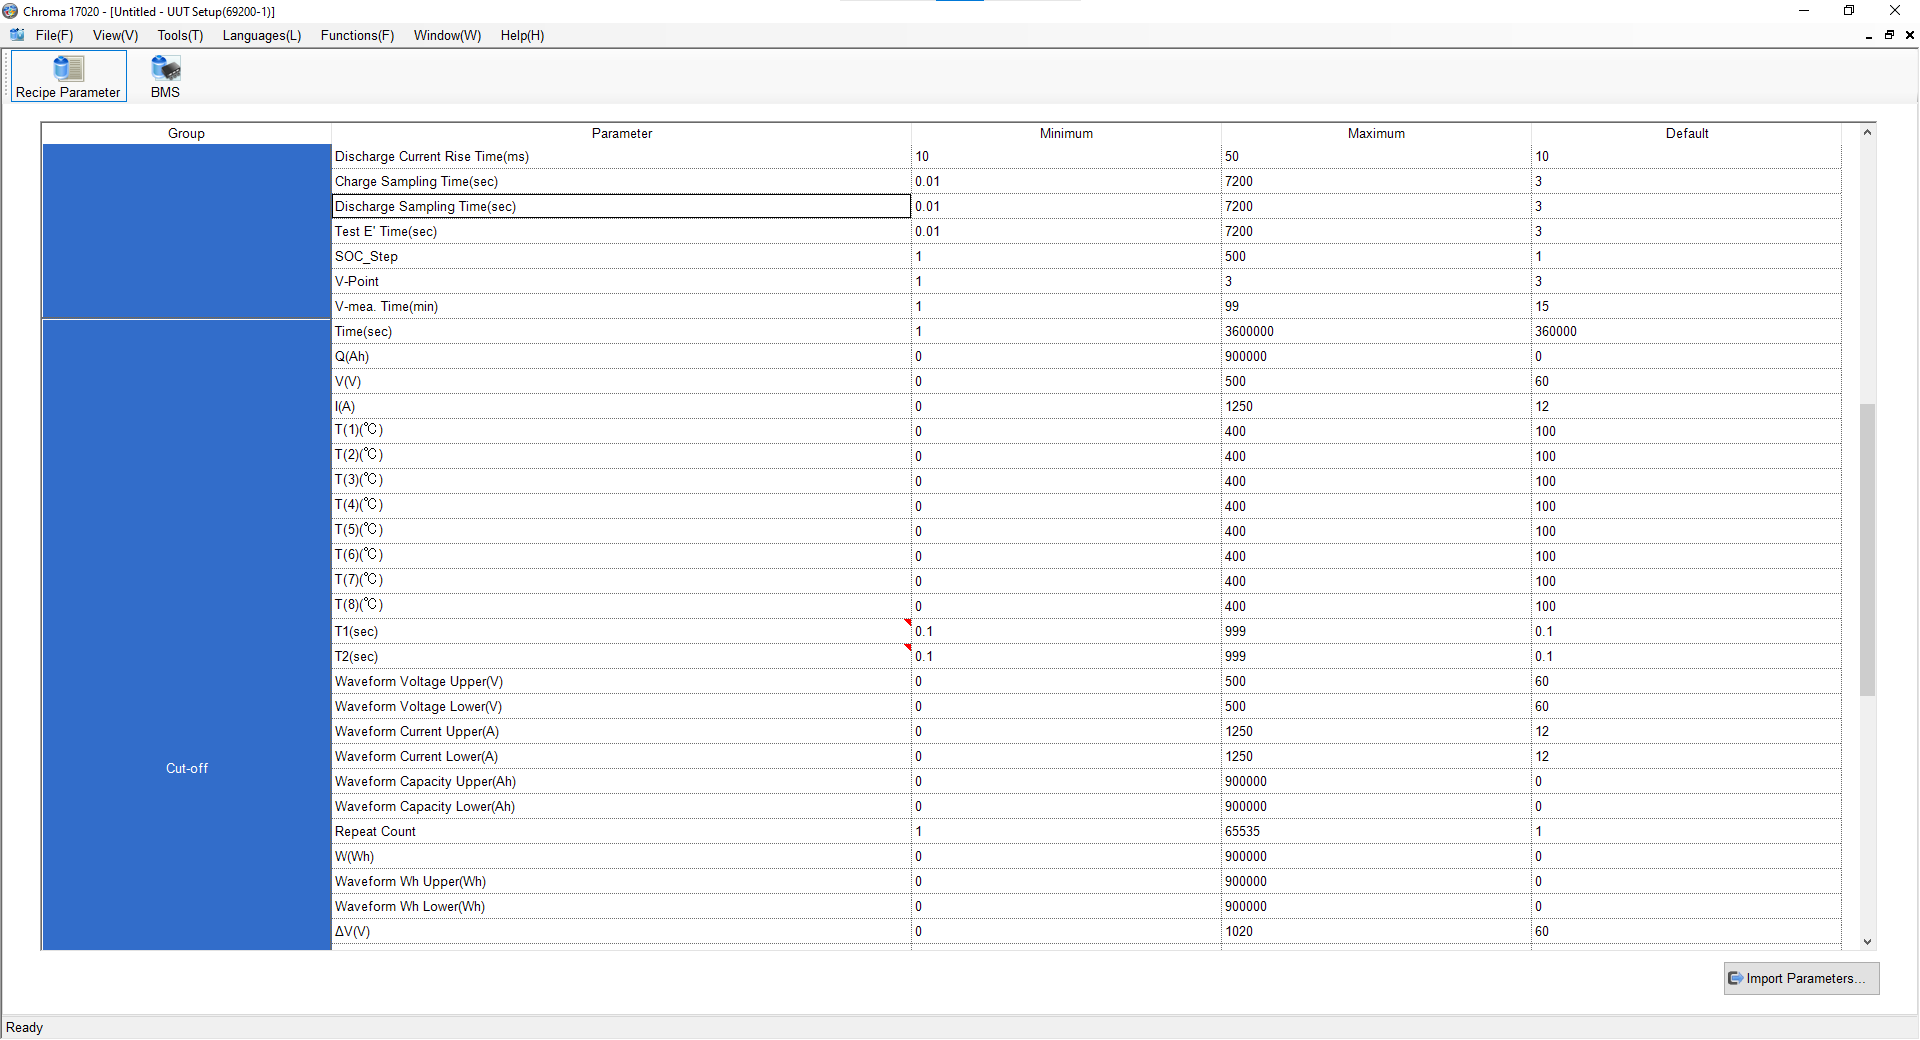
\includegraphics[width=0.8\paperwidth]{Chapters/img/R136_DEMO/UUT_SETUP_2.png}}
		\centering
		\captionsetup{justification=centering,margin=2cm}
		\caption{การกำหนดขอบเขตตัวแปรต่างๆใน UUT Setup (ข)}
		\label{UUT2}
	\end{figure}
	\begin{figure}[H]
	\makebox[\textwidth]{
	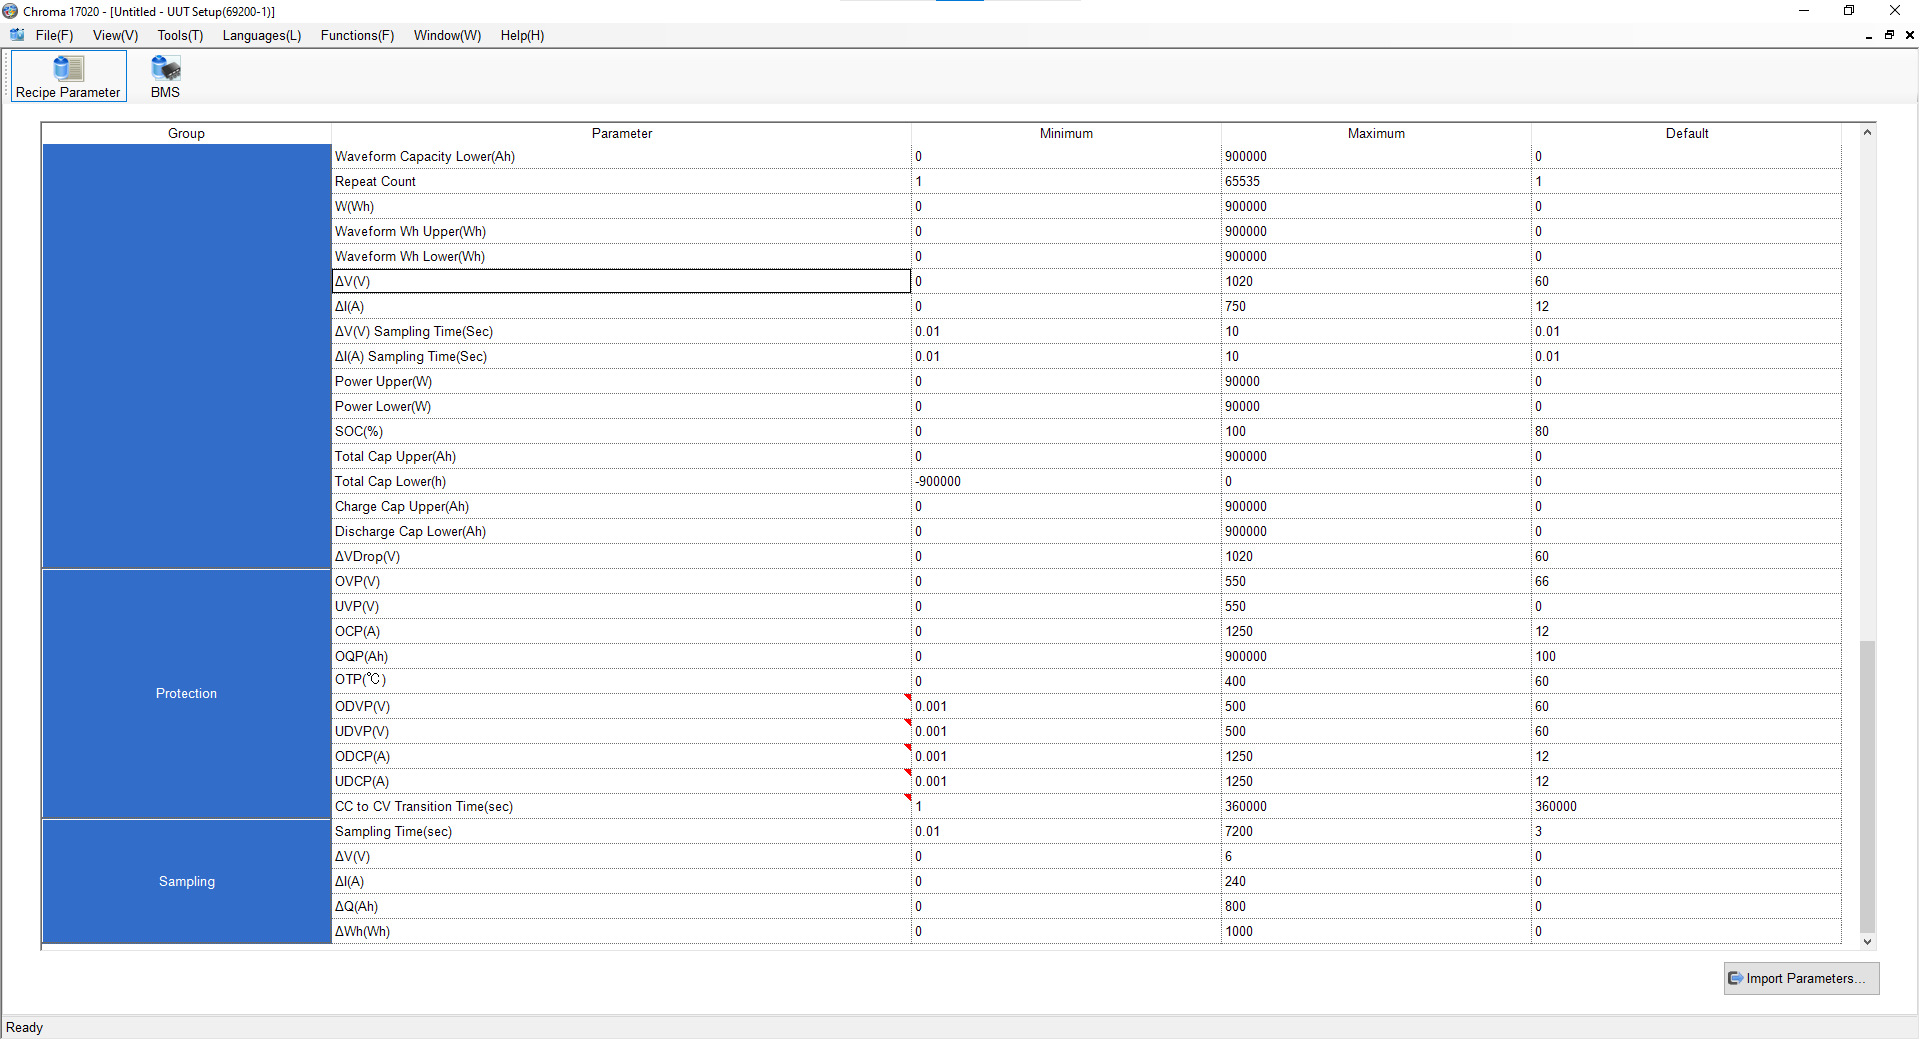
\includegraphics[width=0.8\paperwidth]{Chapters/img/R136_DEMO/UUT_SETUP_3.png}}
		\centering
		\captionsetup{justification=centering,margin=2cm}
		\caption{การกำหนดขอบเขตตัวแปรต่างๆใน UUT Setup (ค)}
		\label{UUT3}
	\end{figure}
\end{center}
\pagebreak
%========================================================================================================
\subsection{การใช้เครื่องทดสอบแบตเตอรี่ Chroma Model 17020 \\ ในการทดสอบการป้องกันการชาร์จเกินของแบตเตอรี่}
สำหรับหัวข้อการทดสอบการป้องกันการชาร์จเกินของแบตเตอรี่โดยใช้เครื่องทดสอบแบตเตอรี่ Chroma Model 17020 ในการทดสอบตัวแปรต่างๆจะถูกตั้งค่าให้เหมาะสมสำหรับการทดสอบตามมาตรฐาน UN ECE Regulation 136 โดยให้เครื่องทดสอบแบตเตอรี่ทำการชาร์จแบตเตอรี่ด้วยอัตรากระแสคงที่ 1/3C ซึ่งเครื่องทดสอบแบตเตอรี่นั้นจะสามารถกำหนดเงื่อนไขเพื่อหยุดทำการทดสอบได้จากขั้นตอนการทดสอบแบตเตอรี่จากมาตรฐาน 
UN ECE Regulation 136 อาจจะทำให้เกิดความเสียหายกับแบตเตอรี่และทรัพย์สินอื่นๆในมหาวิทยาลัยได้ดังนั้นการทดสอบจะไม่ทำตามเงื่อนไขขั้นตอนบางอย่างจากมาตรฐานโดยจะกำหนดเงื่อนไขการทดสอบให้
การทดสอบมีความปลอดภัยมากที่สุดโดยยังคงทดสอบการชาร์จด้วยอัตรากระแสคงที่ 1/3C แต่สำหรับขอบเขตแรงดันที่จะทำให้หยุดการทดสอบนั้นจะกำหนดที่ 86V สำหรับแบตเตอรี่พิกัด 72V 30Ah และแบตเตอรี่พิกัด 72V 60Ah และสุดท้าย 81V สำหรับแบตเตอรี่พิกัด 72V 72Ah โดยค่าตัวแปรต่างๆจะกำหนดค่าดังตารางที่\ref{table:CC_10}-\ref{table:CC_21.6}
\begin{center}
%	\begin{figure}[H]
%		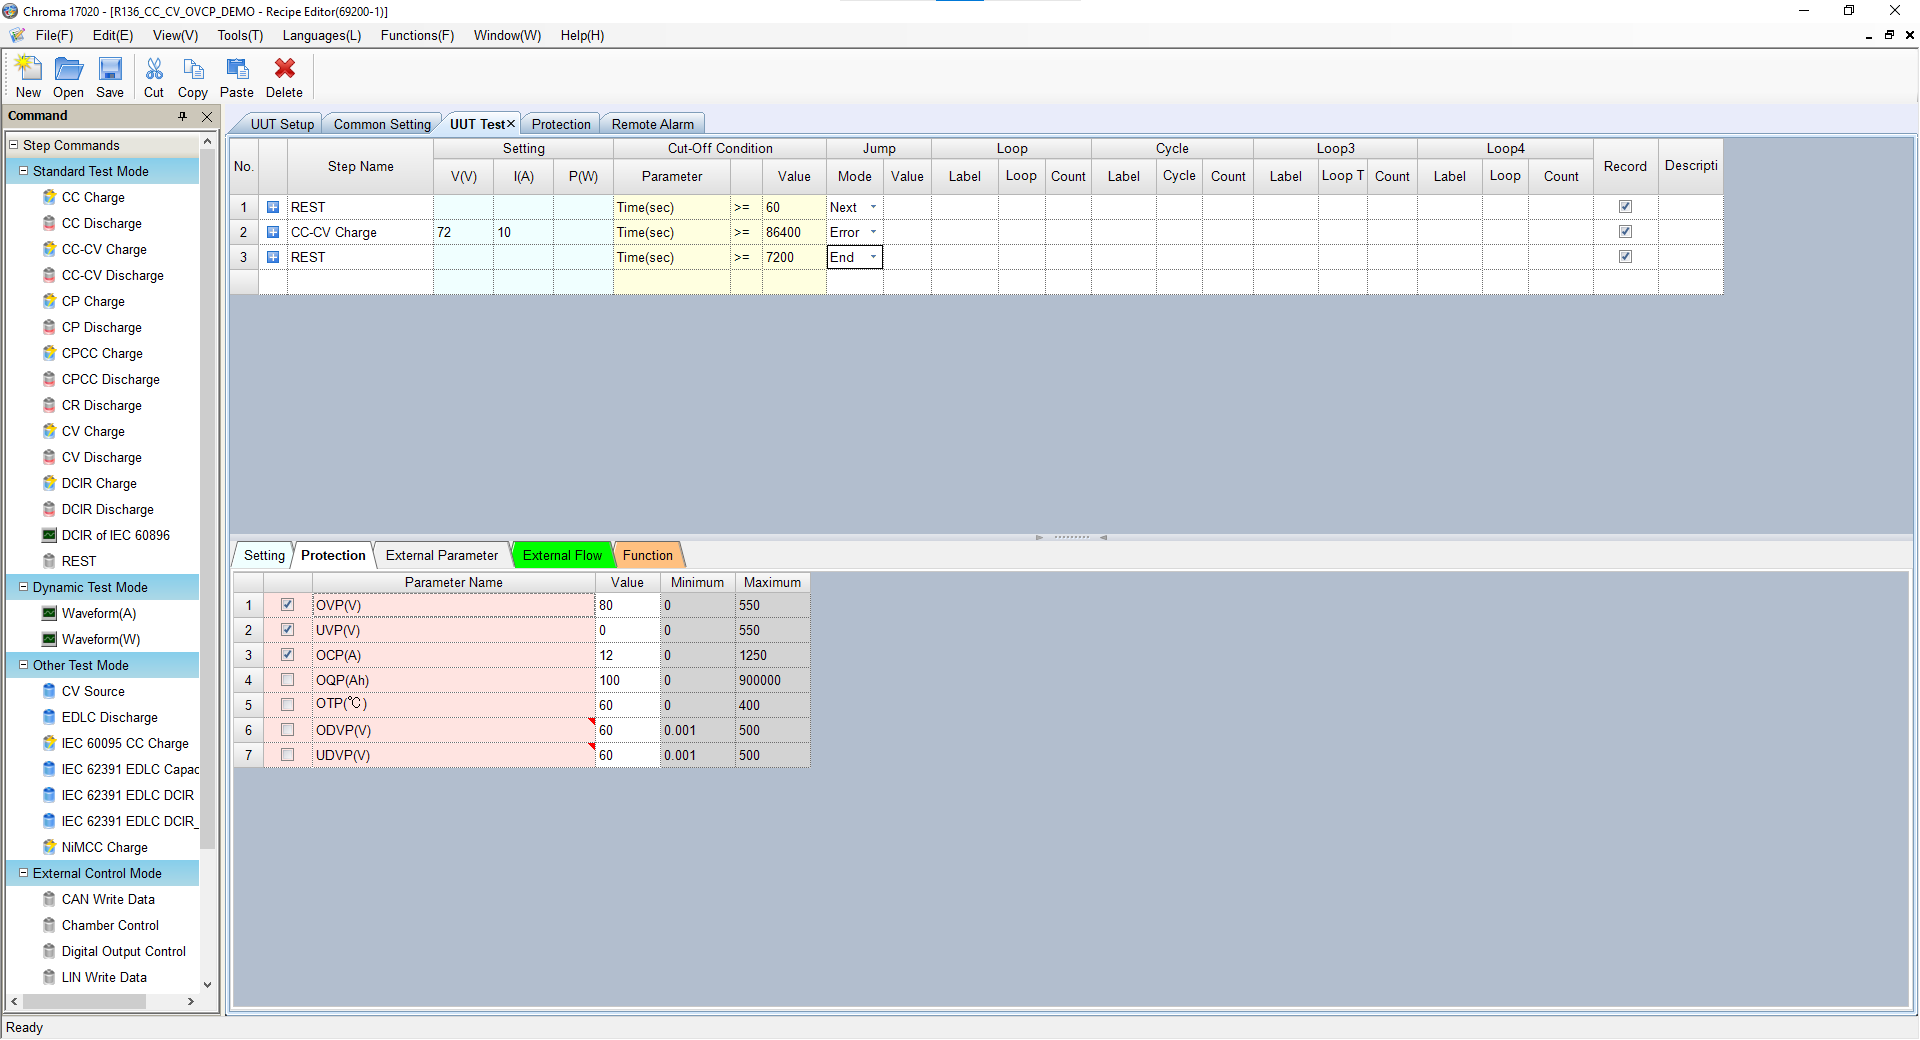
\includegraphics[width=1\linewidth]{Chapters/img/R136_DEMO/UUT_TEST_OVCP.png}
%		\centering
%		\captionsetup{justification=centering,margin=2cm}
%		\caption{การตั้งค่าสำหรับการทดสอบการป้องกันการชาร์จเกินของแบตเตอรี่}
%		\label{fig:setting_charge}
%	\end{figure}
	\begin{figure}[H]
		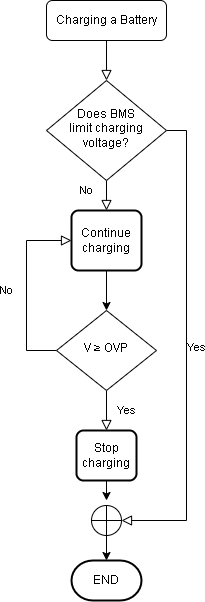
\includegraphics[width=0.25\linewidth]{Chapters/img/R136_DEMO/Charging_flow_chart.png}
		\centering
		\captionsetup{justification=centering,margin=2cm}
		\caption{แผนผังสรุปขั้นตอนการทดสอบการป้องกันการชาร์จเกินของแบตเตอรี่}
	\end{figure}
\end{center}
\begin{table}[H]
\centering
\caption{การตั้งค่าสำหรับการทดสอบการป้องกันการชาร์จเกินของแบตเตอรี่ 72V30Ah}
\resizebox{\textwidth}{!}{%
\begin{tabular}{llllllll}
\hline
\textbf{Step No.} &
  \textbf{Step Information} &
  \textbf{V(V)} &
  \textbf{I(A)} &
  \textbf{P(W)} &
  \textbf{Cut-Off Condition} &
  \textbf{Jump Information} &
  \textbf{Protection} \\ \hline
1 & REST         &  &    &  & Time(sec) \textgreater{}= 60    & Next & OVP(V) = 86 \\
  &              &  &    &  &                                 &      & UVP(V) = 62 \\ 
  &              &  &    &  &                                 &      & OCP(A) = 11 \\ 
2 & CC Charge    &  & 10 &  & Time(sec) \textgreater{}= 11880 & Next &             \\ 
  &              &  &    &  &                                 &      &             \\ 
  &              &  &    &  &                                 &      &             \\ 
3 & REST         &  &    &  & Time(sec) \textgreater{}= 1800  & END  &             \\ \hline
\end{tabular}%
}
\label{table:CC_10}
\end{table}
\begin{table}[H]
\centering
\caption{การตั้งค่าสำหรับการทดสอบการป้องกันการชาร์จเกินของแบตเตอรี่ 72V60Ah}
\resizebox{\textwidth}{!}{%
\begin{tabular}{llllllll}
\hline
\textbf{Step No.} &
  \textbf{Step Information} &
  \textbf{V(V)} &
  \textbf{I(A)} &
  \textbf{P(W)} &
  \textbf{Cut-Off Condition} &
  \textbf{Jump Information} &
  \textbf{Protection} \\ \hline
1 & REST         &  &    &  & Time(sec) \textgreater{}= 60    & Next & OVP(V) = 86 \\
  &              &  &    &  &                                 &      & UVP(V) = 62 \\ 
  &              &  &    &  &                                 &      & OCP(A) = 21 \\ 
2 & CC Charge    &  & 20 &  & Time(sec) \textgreater{}= 11880 & Next &             \\ 
  &              &  &    &  &                                 &      &             \\ 
  &              &  &    &  &                                 &      &             \\ 
3 & REST         &  &    &  & Time(sec) \textgreater{}= 1800  & END  &             \\ \hline
\end{tabular}%
}
\end{table}
\begin{table}[H]
\centering
\caption{การตั้งค่าสำหรับการทดสอบการป้องกันการชาร์จเกินของแบตเตอรี่ 72V72Ah}
\resizebox{\textwidth}{!}{%
\begin{tabular}{llllllll}
\hline
\textbf{Step No.} &
  \textbf{Step Information} &
  \textbf{V(V)} &
  \textbf{I(A)} &
  \textbf{P(W)} &
  \textbf{Cut-Off Condition} &
  \textbf{Jump Information} &
  \textbf{Protection} \\ \hline
1 & REST         &  &    &  & Time(sec) \textgreater{}= 60    & Next & OVP(V) = 81 \\
  &              &  &    &  &                                 &      & UVP(V) = 62 \\ 
  &              &  &    &  &                                 &      & OCP(A) = 23 \\ 
2 & CC Charge    &  &21.6&  & Time(sec) \textgreater{}= 11880 & Next &             \\ 
  &              &  &    &  &                                 &      &             \\ 
  &              &  &    &  &                                 &      &             \\ 
3 & REST         &  &    &  & Time(sec) \textgreater{}= 1800  & END  &             \\ \hline
\end{tabular}%
}
\label{table:CC_21.6}
\end{table}
%========================================================================================================
\subsection{การใช้เครื่องทดสอบแบตเตอรี่ Chroma Model 17020 \\ ในการทดสอบการป้องกันการดิสชาร์จเกินของแบตเตอรี่}
เช่นเดียวกับหัวข้อที่ผ่านมาสำหรับหัวข้อการทดสอบการป้องกันการดิสชาร์จเกินของแบตเตอรี่โดยใช้เครื่องทดสอบแบตเตอรี่ Chroma Model 17020 ในการทดสอบตัวแปรต่างๆจะถูกตั้งค่าให้เหมาะสมสำหรับ
การทดสอบตามมาตรฐาน UN ECE Regulation 136 โดยให้เครื่องทดสอบแบตเตอรี่ทำการดิสชาร์จแบตเตอรี่ด้วยอัตรากระแสคงที่ 1/3C แต่สำหรับแบตเตอรี่ 72V 72Ah จะใช้อัตรากระแส 0.5C ซึ่งเครื่องทดสอบแบตเตอรี่นั้นจะสามารถกำหนดเงื่อนไขเพื่อหยุดทำการทดสอบได้เช่นกันโดยการทดสอบนี้จะไม่ทำตามเงื่อนไขขั้นตอนบางอย่างจากมาตรฐานโดยจะกำหนดเงื่อนไขการทดสอบให้
การทดสอบมีความปลอดภัยมากที่สุดโดยยังคงทดสอบการดิสชาร์จด้วยอัตรากระแสคงที่ 1/3C (0.5C สำหรับแบตเตอรี่ 72V 72Ah)แต่สำหรับขอบเขตแรงดันที่จะทำให้หยุดการทดสอบนั้นจะกำหนดที่ 
56V สำหรับแบตเตอรี่พิกัด 72V 30Ah และแบตเตอรี่พิกัด 72V 60Ah และสุดท้าย 57V สำหรับแบตเตอรี่พิกัด 72V 72Ah โดยค่าตัวแปรต่างๆจะกำหนดค่าดังตารางที่
\ref{table:CC_D_10}-\ref{table:CC_D_36}
\begin{center}
%	\begin{figure}[H]
%		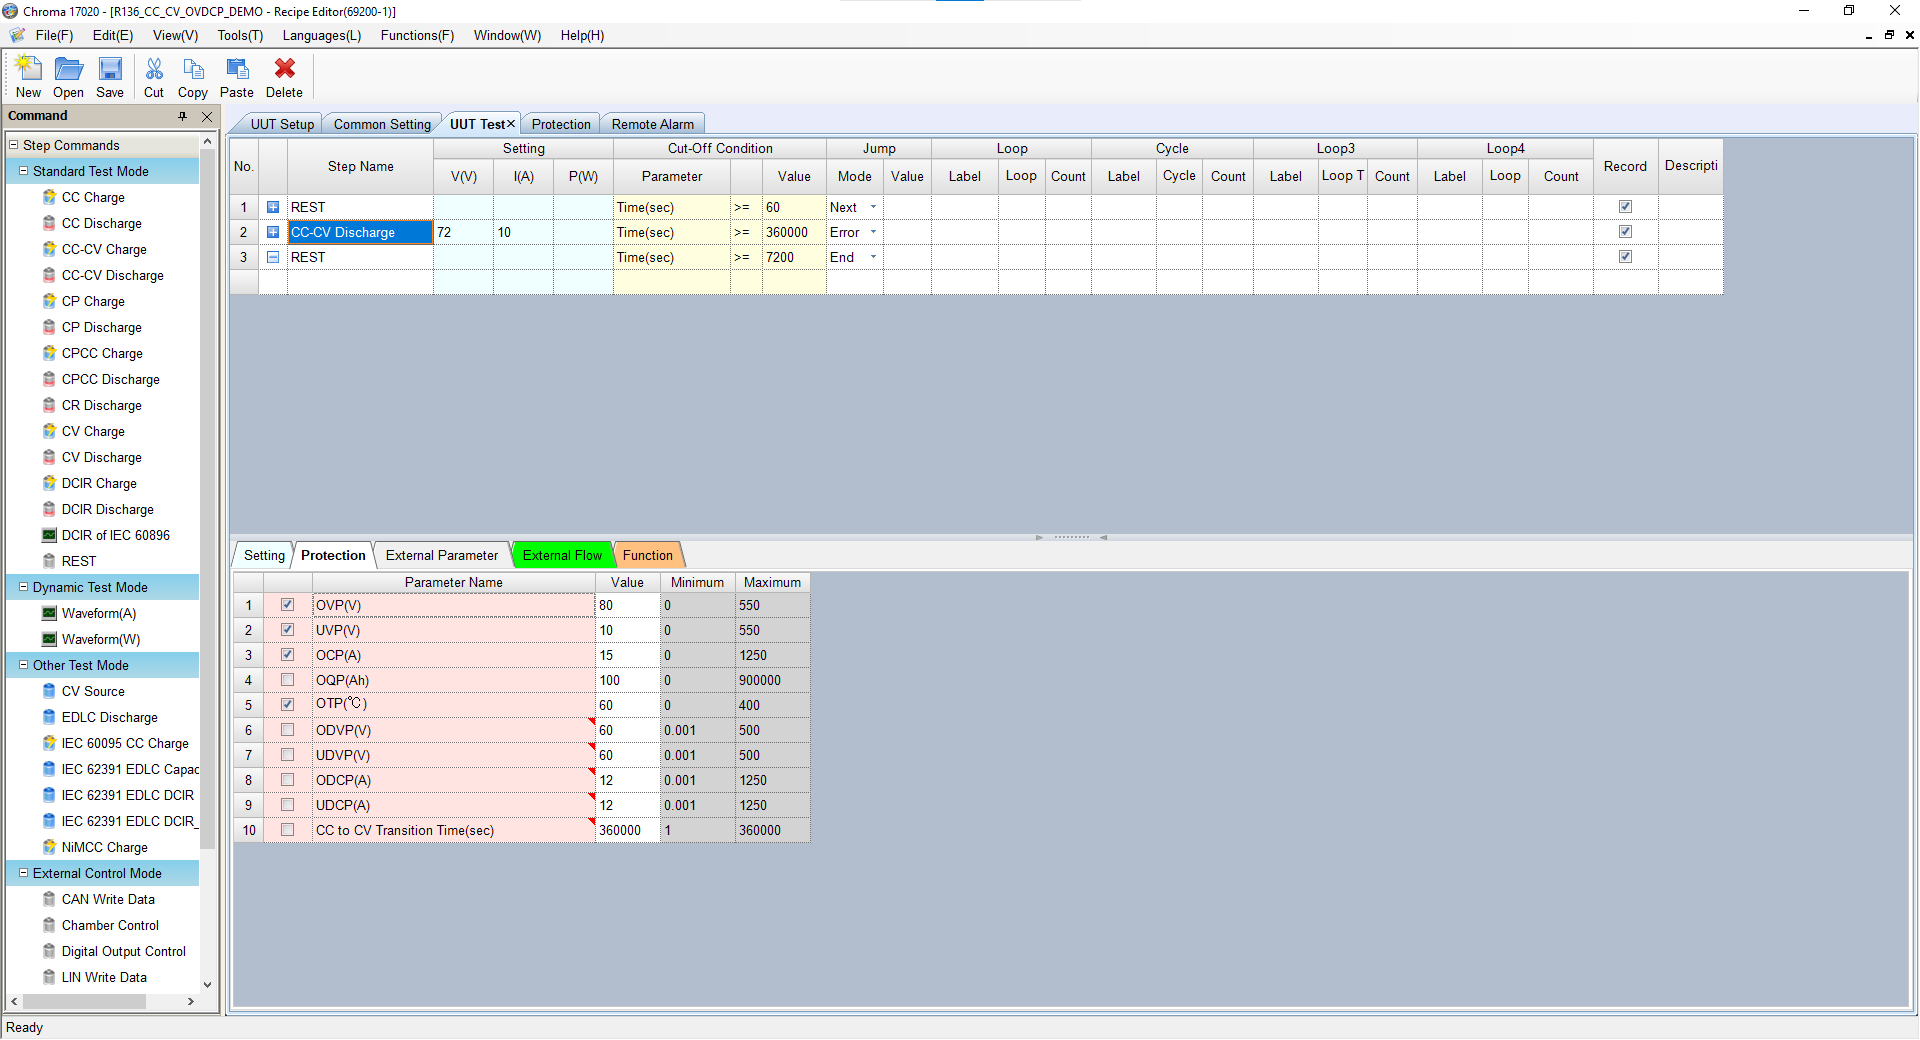
\includegraphics[width=1\linewidth]{Chapters/img/R136_DEMO/UUT_TEST_OVDCP.png}
%		\centering
%		\captionsetup{justification=centering,margin=2cm}
%		\caption{การตั้งค่าสำหรับการทดสอบการป้องกันการดิสชาร์จเกินของแบตเตอรี่}
%		\label{fig:setting_discharge}
%	\end{figure}
	\begin{figure}[H]
		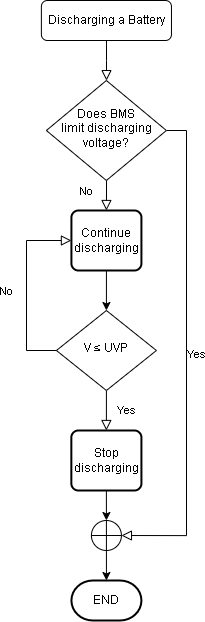
\includegraphics[width=0.25\linewidth]{Chapters/img/R136_DEMO/Discharging_flow_chart.png}
		\centering
		\captionsetup{justification=centering,margin=2cm}
		\caption{แผนผังสรุปขั้นตอนการทดสอบการป้องกันการดิสชาร์จเกินของแบตเตอรี่}
	\end{figure}
\end{center}
\begin{table}[H]
\centering
\caption{การตั้งค่าสำหรับการทดสอบการป้องกันการดิสชาร์จเกินของแบตเตอรี่ 72V30Ah}
\resizebox{\textwidth}{!}{%
\begin{tabular}{llllllll}
\hline
\textbf{Step No.} &
  \textbf{Step Information} &
  \textbf{V(V)} &
  \textbf{I(A)} &
  \textbf{P(W)} &
  \textbf{Cut-Off Condition} &
  \textbf{Jump Information} &
  \textbf{Protection} \\ \hline
1 & REST         &  &    &  & Time(sec) \textgreater{}= 60    & Next & OVP(V) = 86 \\ 
  &              &  &    &  &                                 &      & UVP(V) = 53 \\ 
  &              &  &    &  &                                 &      & OCP(A) = 11 \\ 
2 & CC Discharge &  & 10 &  & Time(sec) \textgreater{}= 11880 & Next &             \\ 
  &              &  &    &  & V(V) \textless 56               & Next &             \\ 
  &              &  &    &  &                                 &      &             \\ 
3 & REST         &  &    &  & Time(sec) \textgreater{}= 1800  & END  &             \\ \hline
\end{tabular}%
}
\label{table:CC_D_10}
\end{table}
\begin{table}[H]
\centering
\caption{การตั้งค่าสำหรับการทดสอบการป้องกันการดิสชาร์จเกินของแบตเตอรี่ 72V60Ah}
\resizebox{\textwidth}{!}{%
\begin{tabular}{llllllll}
\hline
\textbf{Step No.} &
  \textbf{Step Information} &
  \textbf{V(V)} &
  \textbf{I(A)} &
  \textbf{P(W)} &
  \textbf{Cut-Off Condition} &
  \textbf{Jump Information} &
  \textbf{Protection} \\ \hline
1 & REST         &  &    &  & Time(sec) \textgreater{}= 60    & Next & OVP(V) = 86 \\ 
  &              &  &    &  &                                 &      & UVP(V) = 53 \\ 
  &              &  &    &  &                                 &      & OCP(A) = 21 \\ 
2 & CC Discharge &  & 20 &  & Time(sec) \textgreater{}= 11880 & Next &             \\ 
  &              &  &    &  & V(V) \textless 56               & Next &             \\ 
  &              &  &    &  &                                 &      &             \\ 
3 & REST         &  &    &  & Time(sec) \textgreater{}= 1800  & END  &             \\ \hline
\end{tabular}%
}
\end{table}
\begin{table}[H]
\centering
\caption{การตั้งค่าสำหรับการทดสอบการป้องกันการดิสชาร์จเกินของแบตเตอรี่ 72V72Ah}
\resizebox{\textwidth}{!}{%
\begin{tabular}{llllllll}
\hline
\textbf{Step No.} &
  \textbf{Step Information} &
  \textbf{V(V)} &
  \textbf{I(A)} &
  \textbf{P(W)} &
  \textbf{Cut-Off Condition} &
  \textbf{Jump Information} &
  \textbf{Protection} \\ \hline
1 & REST         &  &    &  & Time(sec) \textgreater{}= 60    & Next & OVP(V) = 81 \\ 
  &              &  &    &  &                                 &      & UVP(V) = 53 \\ 
  &              &  &    &  &                                 &      & OCP(A) = 37 \\ 
2 & CC Discharge &  & 36 &  & Time(sec) \textgreater{}= 11880 & Next &             \\ 
  &              &  &    &  & V(V) \textless 56               & Next &             \\ 
  &              &  &    &  &                                 &      &             \\ 
3 & REST         &  &    &  & Time(sec) \textgreater{}= 1800  & END  &             \\ \hline
\end{tabular}%
}
\label{table:CC_D_36}
\end{table}

%========================================================================================================
\subsection{การใช้เครื่องทดสอบแบตเตอรี่ Chroma Model 17020 \\ ในการทดสอบอื่นๆ}
สำหรับการทดสอบการวัดค่าความต้านภายในของแบตเตอรี่จะทดสอบเฉพาะแบตเตอรี่พิกัด 72V 72Ah โดยจะดิสชาร์จด้วยกระแสคงที่ 0.2C เป็นระยะเวลา 10 วินาทีจากนั้นจะดิสชาร์จด้วยกระแสคงที่ 
1C เป็นระยะเวลา 1 วินาทีโดยการกำหนดตัวแปรต่างๆจะเป็นไปดังรูปที่\ref{table:DCIR} และสำหรับการทดสอบระยะเวลาการพักและทดสอบอัตรากระแสจะสังเกตจากการทดสอบก่อนหน้านี้จากการตั้งค่าดังตารางที่
\ref{table:CC_D_36} และทดสอบโดยเปรียบเทียบการทดสอบโดยการตั้งค่าดังตารางที่\ref{table:CC_D_21.6} เพื่อทดสอบอัตรากระแสที่มีผลต่อความจุและสุดท้ายสำหรับการทดสอบระยะเวลาในการพัก
จะตั้งค่าดังตารางที่\ref{table:CC_D_36}
\begin{center}
%	\begin{figure}[H]
%		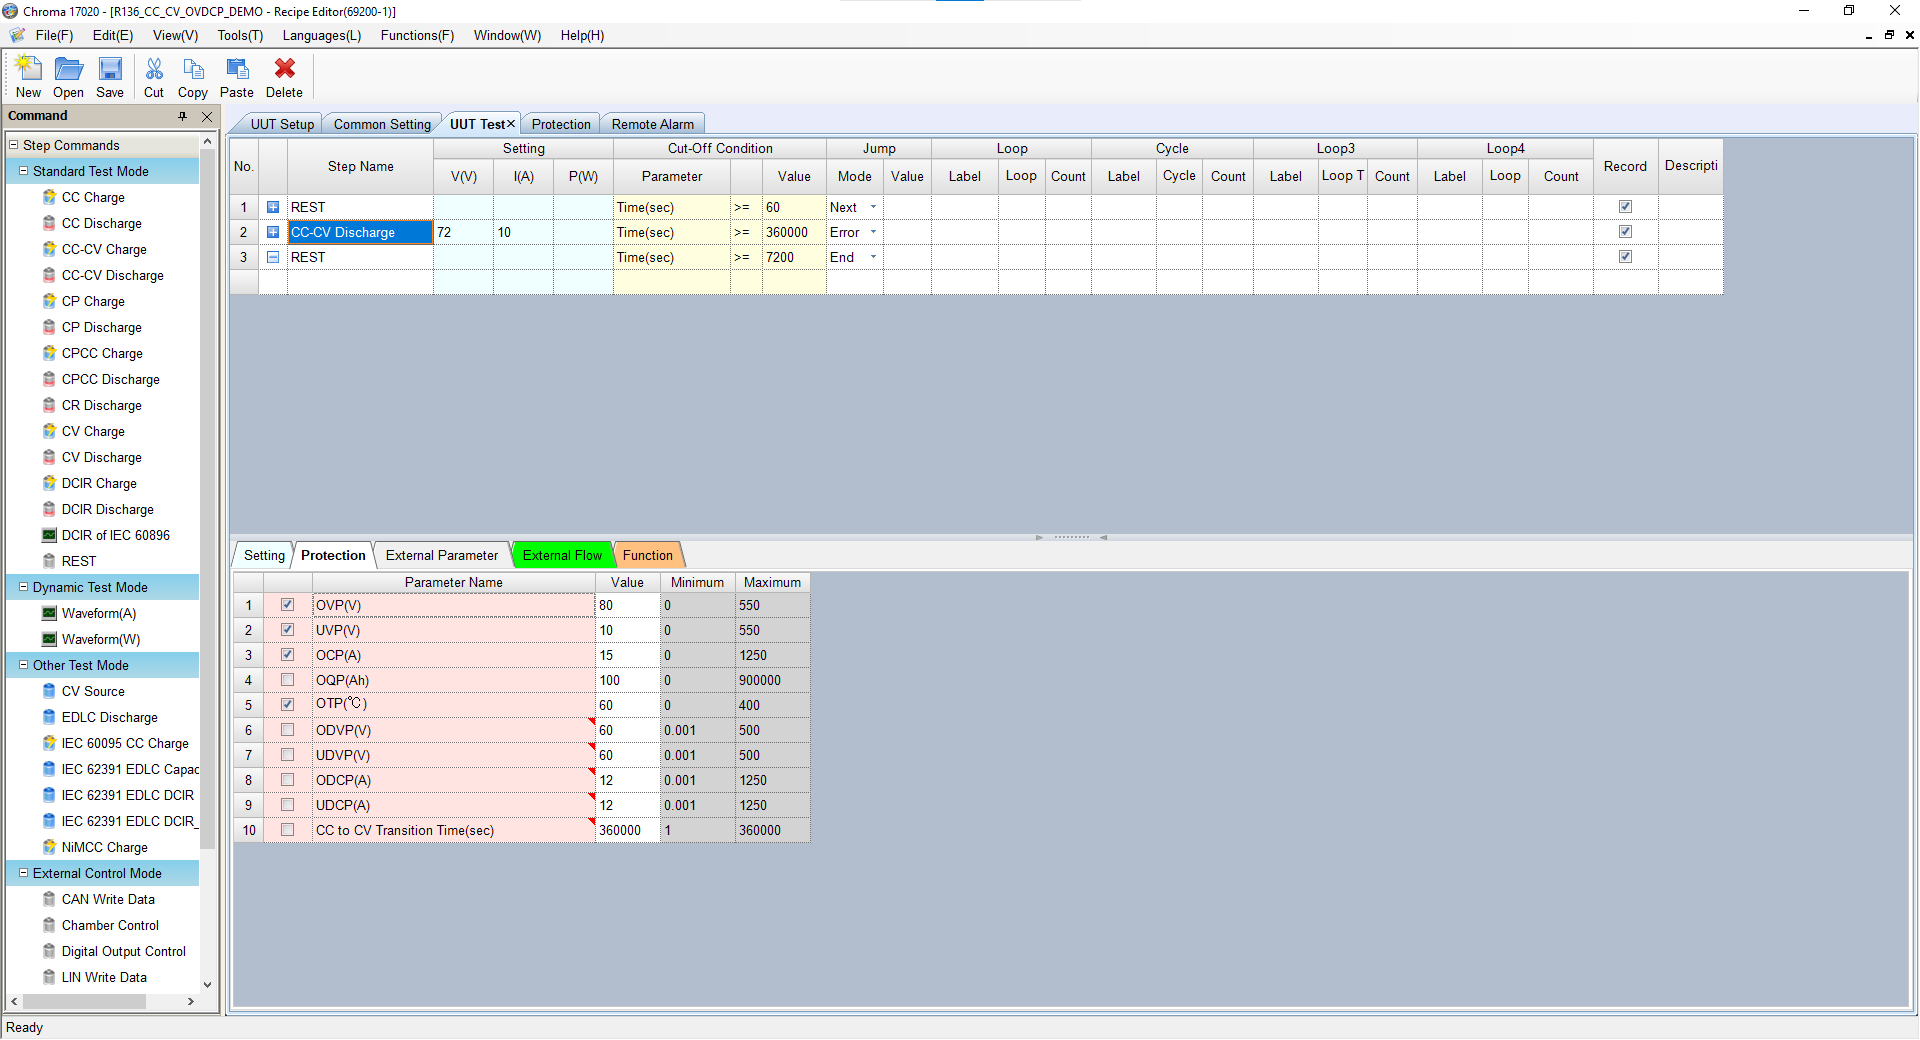
\includegraphics[width=1\linewidth]{Chapters/img/R136_DEMO/UUT_TEST_OVDCP.png}
%		\centering
%		\captionsetup{justification=centering,margin=2cm}
%		\caption{การตั้งค่าสำหรับการทดสอบการป้องกันการดิสชาร์จเกินของแบตเตอรี่}
%		\label{fig:setting_rest}
%	\end{figure}


\begin{table}[H]
\centering
\caption{การตั้งค่าสำหรับการทดสอบวัดค่าความต้านทานภายในของแบตเตอรี่ 72V72Ah}
\resizebox{\textwidth}{!}{%
\begin{tabular}{llllllll}
\hline
\textbf{Step No.} &
  \textbf{Step Information} &
  \textbf{V(V)} &
  \textbf{I(A)} &
  \textbf{P(W)} &
  \textbf{Cut-Off Condition} &
  \textbf{Jump Information} &
  \textbf{Protection} \\ \hline
1 & REST &  &  &  & Time(sec) \textgreater{}= 10 & Next & OVP(V) = 86 \\ 
  &      &  &  &  &                              &      & UVP(V) = 53 \\ 
2 & DCIR &  &  &  & Time(sec) \textgreater{}= 21 & Next &             \\ 
  &      &  &  &  &                              &      &             \\ 
1 & REST &  &  &  & Time(sec) \textgreater{}= 60 & Next &             \\ 
  &      &  &  &  &                              &      &             \\ \hline
\end{tabular}%
}
\label{table:DCIR}
\end{table}

\begin{table}[H]
\centering
\caption{การตั้งค่าสำหรับการทดสอบการดิสชาร์จที่ 0.3C สำหรับแบตเตอรี่ 72V72Ah}
\resizebox{\textwidth}{!}{%
\begin{tabular}{llllllll}
\hline
\textbf{Step No.} &
  \textbf{Step Information} &
  \textbf{V(V)} &
  \textbf{I(A)} &
  \textbf{P(W)} &
  \textbf{Cut-Off Condition} &
  \textbf{Jump Information} &
  \textbf{Protection} \\ \hline
1 & REST         &  &    &  & Time(sec) \textgreater{}= 60    & Next & OVP(V) = 81 \\ 
  &              &  &    &  &                                 &      & UVP(V) = 53 \\ 
  &              &  &    &  &                                 &      & OCP(A) = 37 \\ 
2 & CC Discharge &  &21.6&  & Time(sec) \textgreater{}= 11880 & Next &             \\ 
  &              &  &    &  & V(V) \textless 56               & Next &             \\ 
  &              &  &    &  &                                 &      &             \\ 
3 & REST         &  &    &  & Time(sec) \textgreater{}= 1800  & END  &             \\ \hline
\end{tabular}%
}
\label{table:CC_D_21.6}
\end{table}
\end{center}









